\mysection{\HelloWorldSectionName}
\label{sec:helloworld}

Продолжим, используя знаменитый пример из книги [\KRBook]:

\lstinputlisting[caption=код на Си/Си++,style=customc]{patterns/01_helloworld/hw.c}

\subsection{x86}

\EN{\subsubsection{MSVC}

Let's compile it in MSVC 2010:

\begin{lstlisting}
cl 1.cpp /Fa1.asm
\end{lstlisting}

(The \TT{/Fa} option instructs the compiler to generate an assembly listing file)

\begin{lstlisting}[caption=MSVC 2010,style=customasmx86]
CONST	SEGMENT
$SG3830	DB	'hello, world', 0AH, 00H
CONST	ENDS
PUBLIC	_main
EXTRN	_printf:PROC
; Function compile flags: /Odtp
_TEXT	SEGMENT
_main	PROC
	push	ebp
	mov	ebp, esp
	push	OFFSET $SG3830
	call	_printf
	add	esp, 4
	xor	eax, eax
	pop	ebp
	ret	0
_main	ENDP
_TEXT	ENDS
\end{lstlisting}

MSVC produces assembly listings in Intel-syntax.
The differences between Intel-syntax and AT\&T-syntax will be discussed in \myref{ATT_syntax}.

The compiler generated the file, \TT{1.obj}, which is to be linked into \TT{1.exe}.
In our case, the file contains two segments: \TT{CONST} (for data constants) and \TT{\_TEXT} (for code).

\myindex{\CLanguageElements!const}
\label{string_is_const_char}
The string \TT{hello, world} in \CCpp has type \TT{const char[]}\InSqBrackets{\TCPPPL p176, 7.3.2}, but it does not have its own name.
The compiler needs to deal with the string somehow, so it defines the internal name \TT{\$SG3830} for it.

That is why the example may be rewritten as follows:

\lstinputlisting[style=customc]{patterns/01_helloworld/hw_2.c}

Let's go back to the assembly listing. As we can see, the string is terminated by a zero byte, which is standard for \CCpp strings.
More about \CCpp strings: \myref{C_strings}.

In the code segment, \TT{\_TEXT}, there is only one function so far: \main{}.
The function \main starts with prologue code and ends with epilogue code (like almost any function)
\footnote{You can read more about it in the section about function prologues and epilogues ~(\myref{sec:prologepilog}).}.

\myindex{x86!\Instructions!CALL}
After the function prologue we see the call to the \printf{} function:\\
\INS{CALL \_printf}.
\myindex{x86!\Instructions!PUSH}
Before the call, a string address (or a pointer to it) containing our greeting is placed on the stack with the help of the \PUSH instruction.

When the \printf function returns the control to the \main function, the string address (or a pointer to it) is still on the stack.
Since we do not need it anymore, the \gls{stack pointer} (the \ESP register) needs to be corrected.

\myindex{x86!\Instructions!ADD}
\INS{ADD ESP, 4} means add 4 to the \ESP register value.

Why 4? Since this is a 32-bit program, we need exactly 4 bytes for address passing through the stack. If it was x64 code we would need 8 bytes.
\INS{ADD ESP, 4} is effectively equivalent to \INS{POP register} but without using any register\footnote{CPU flags, however, are modified}.

\myindex{Intel C++}
\myindex{\oracle}
\myindex{x86!\Instructions!POP}

For the same purpose, some compilers (like the Intel C++ Compiler) may emit \TT{POP ECX}
instead of \ADD (e.g., such a pattern can be observed in the \oracle{} code as it is compiled with the Intel C++ compiler).
This instruction has almost the same effect but the \ECX register contents will be overwritten.
The Intel C++ compiler supposedly uses \TT{POP ECX} since this instruction's opcode is shorter than \TT{ADD ESP, x} (1 byte for \TT{POP} against 3 for \TT{ADD}).

Here is an example of using \POP instead of \ADD from \oracle{}:

\begin{lstlisting}[caption=\oracle 10.2 Linux (app.o file),style=customasmx86]
.text:0800029A                 push    ebx
.text:0800029B                 call    qksfroChild
.text:080002A0                 pop     ecx
\end{lstlisting}

However, MSVC can do the same.

\begin{lstlisting}[caption=MineSweeper from Windows 7 32-bit]
.text:0102106F                 push    0
.text:01021071                 call    ds:time
.text:01021077                 pop     ecx
\end{lstlisting}

%Read more about the stack in section
% ~(\myref{sec:stack}).
\myindex{\CLanguageElements!return}
After calling \printf, the original \CCpp code contains the statement \TT{return 0}~---return 0 as the result of the \main function.

\myindex{x86!\Instructions!XOR}
In the generated code this is implemented by the instruction \INS{XOR EAX, EAX}.

\myindex{x86!\Instructions!MOV}

\XOR is in fact just \q{eXclusive OR}\footnote{\href{http://en.wikipedia.org/wiki/Exclusive_or}{Wikipedia}} but the compilers often use it instead of
\INS{MOV EAX, 0}---again because it is a slightly shorter opcode (2 bytes for \XOR against 5 for \MOV).

\myindex{x86!\Instructions!SUB}
Some compilers emit \INS{SUB EAX, EAX}, which means \emph{SUBtract the value in the} \EAX \emph{from the value in} \EAX. That in any case will results in zero.

\myindex{x86!\Instructions!RET}
The last instruction \RET returns the control to the \gls{caller}. Usually, this is \CCpp \ac{CRT} code which in turn returns control to the \ac{OS}.
}
\FR{\subsubsection{MSVC}

Compilons-le avec MSVC 2010:

\begin{lstlisting}
cl 1.cpp /Fa1.asm
\end{lstlisting}

(L'option \TT{/Fa} indique au compilateur de générer un fichier avec le listing en assembleur)

\begin{lstlisting}[caption=MSVC 2010,style=customasmx86]
CONST	SEGMENT
$SG3830	DB	'hello, world', 0AH, 00H
CONST	ENDS
PUBLIC	_main
EXTRN	_printf:PROC
; Function compile flags: /Odtp
_TEXT	SEGMENT
_main	PROC
	push	ebp
	mov	ebp, esp
	push	OFFSET $SG3830
	call	_printf
	add	esp, 4
	xor	eax, eax
	pop	ebp
	ret	0
_main	ENDP
_TEXT	ENDS
\end{lstlisting}

MSVC génère des listings assembleur avec la syntaxe Intel.
La différence entre la syntaxe Intel et la syntaxe AT\&T sera discutée dans \myref{ATT_syntax}.

Le compilateur a généré le fichier object \TT{1.obj}, qui sera lié dans l'exécutable \TT{1.exe}.
Dans notre cas, le fichier contient deux segments: \TT{CONST} (pour les données constantes)
 et \TT{\_TEXT} (pour le code).

\myindex{\CLanguageElements!const}
\label{string_is_const_char}
La chaîne \TT{hello, world} en \CCpp a le type \TT{const char[]}\InSqBrackets{\TCPPPL p176, 7.3.2}, mais
elle n'a pas de nom.
Le compilateur doit pouvoir l'utiliser et lui défini donc le nom interne \TT{\$SG3830} à cette fin.

C'est pourquoi l'exemple pourrait être récrit comme suit:

\lstinputlisting[style=customc]{patterns/01_helloworld/hw_2.c}

Retournons au listing assembleur. Comme nous le voyons, la chaîne est terminée avec un octet à zéro, ce qui
est le standard pour les chaînes \CCpp.

Dans le segment de code, \TT{\_TEXT}, il n'y a qu'une seule fonction: \main{}.
La fonction \main débute par le code du prologue et se termine par le code de l'épilogue 
(comme presque toutes les fonctions)
\footnote{Vous pouvez en lire plus dans la section concernant les prologues et épilogues de
fonctions ~(\myref{sec:prologepilog}).}.

\myindex{x86!\Instructions!CALL}
Après le prologue de la fonction nous voyons l'appel à la fonction \printf{}:\\
\INS{CALL \_printf}.
\myindex{x86!\Instructions!PUSH}
Avant l'appel, l'adresse de la chaîne (ou un pointeur sur elle) contenant notre message
 est placée sur la pile avec l'aide de l'instruction \PUSH.

Lorsque la fonction \printf rend le contrôle à la fonction \main, l'adresse de la chaîne (ou un pointeur sur elle)
est toujours sur la pile.
Comme nous n'en avons plus besoin, le pointeur de pile (\gls{stack pointer} le registre \ESP) doit être corrigé.

\myindex{x86!\Instructions!ADD}
\INS{ADD ESP, 4} signifie ajouter 4 à la valeur du registre \ESP.

Pourquoi 4? puisqu'il s'agit d'un programme 32-bit, nous avons besoin d'exactement 4 octets pour passer une adresse
par la pile. S'il s'agissait d'un code x64, nous aurions besoin de 8 octets.
\INS{ADD ESP, 4} est effectivement équivalent à \INS{POP register} mais sans utiliser de registre\footnote{Les
flags du CPU, toutefois, sont modifiés}.

\myindex{Intel C++}
\myindex{\oracle}
\myindex{x86!\Instructions!POP}

Pour la même raison, certains compilateurs (comme le compilateur C++ d'Intel) peuvent générer \TT{POP ECX}
à la place de \ADD (e.g., ce comportement peut être observé dans le code d'\oracle{} car il est
compilé avec le compilateur C++ d'Intel.
Cette instruction a presque le même effet mais le contenu du registre \ECX sera écrasé.
Le compilateur C++ d'Intel utilise probablement \TT{POP ECX} car l'opcode de cette instruction est plus
 court que celui de \TT{ADD ESP, x} (1 octet pour \TT{POP} contre 3 pour \TT{ADD}).

Voici un exemple d'utilisation de \POP à la place de \ADD dans \oracle{}:

\begin{lstlisting}[caption=\oracle 10.2 Linux (app.o file),style=customasmx86]
.text:0800029A                 push    ebx
.text:0800029B                 call    qksfroChild
.text:080002A0                 pop     ecx
\end{lstlisting}

Toutefois, MSVC peut faire de même.

\begin{lstlisting}[caption=MineSweeper de Windows 7 32-bit]
.text:0102106F                 push    0
.text:01021071                 call    ds:time
.text:01021077                 pop     ecx
\end{lstlisting}

%Lisez en plus à propos de la pile dans la section
% ~(\myref{sec:stack}).

\myindex{\CLanguageElements!return}
Après l'appel de \printf, le code \CCpp original contient la déclaration \TT{return 0}~---renvoie 0 comme valeur de retour de la fonction \main.

\myindex{x86!\Instructions!XOR}
Dans le code généré cela est implémenté par l'instruction \INS{XOR EAX, EAX}.

\myindex{x86!\Instructions!MOV}

\XOR est en fait un simple \q{OU exclusif (eXclusive OR}\footnote{\href{http://en.wikipedia.org/wiki/Exclusive_or}{Wikipédia}} mais
les compilateurs l'utilisent souvent à la place de \INS{MOV EAX, 0}---à nouveau parce que l'opcode est légèrement plus
court (2 octets pour \XOR contre 5 pour \MOV).

\myindex{x86!\Instructions!SUB}
Certains compilateurs génèrent \INS{SUB EAX, EAX}, qui signifie \emph{Soustraire la valeur dans} \EAX \emph{de la valeur dans} \EAX,
 ce qui, dans tous les cas, donne zéro.

\myindex{x86!\Instructions!RET}
La dernière instruction \RET redonne le contrôle à l'\glslink{caller}{appelant}.
Habituellement, c'est ce code \CCpp \ac{CRT}, qui, à son tour, redonne le contrôle à l'\ac{OS}.

}
\IT{\subsubsection{MSVC}

Compiliamolo in MSVC 2010:

\begin{lstlisting}
cl 1.cpp /Fa1.asm
\end{lstlisting}

(l'opzione \TT{/Fa} indica al compilatore di generare un file con il listato assembly)

\begin{lstlisting}[caption=MSVC 2010,style=customasmx86]
CONST	SEGMENT
$SG3830	DB	'hello, world', 0AH, 00H
CONST	ENDS
PUBLIC	_main
EXTRN	_printf:PROC
; Function compile flags: /Odtp
_TEXT	SEGMENT
_main	PROC
	push	ebp
	mov	ebp, esp
	push	OFFSET $SG3830
	call	_printf
	add	esp, 4
	xor	eax, eax
	pop	ebp
	ret	0
_main	ENDP
_TEXT	ENDS
\end{lstlisting}

MSVC produce codice assembly in sintassi Intel.
La differenza tra le sintassi Intel e AT\&T-syntax sarà discussa al \myref{ATT_syntax}.

Il compilatore ha generato il file, \TT{1.obj}, che deve essere linkato in \TT{1.exe}.
Nel nostro caso, il file contiene due segmenti: \TT{CONST} (per i dati constanti) e \TT{\_TEXT} (per il codice).

\myindex{\CLanguageElements!const}
\label{string_is_const_char}
La stringa \TT{hello, world} in \CCpp ha tipo \TT{const char[]}\InSqBrackets{\TCPPPL p176, 7.3.2}, ma non ha un nome assegnato.
Il compilatore deve in qualche modo aver a che fare con la stringa, e la definisce quindi con il nome interno \TT{\$SG3830}.

Questo è il motivo per cui l'esempio potrebbe essere riscritto nel modo seguente:

\lstinputlisting[style=customc]{patterns/01_helloworld/hw_2.c}

Torniamo al listato assembly. Come possiamo vedere, la stringa è terminata con un byte zero, che è lo standard per la terminazione delle stringhe \CCpp.
Più informazioni sulle stringhe in \CCpp: \myref{C_strings}.

Nel code segment, \TT{\_TEXT}, esiste fino ad ora solo una funzione: \main{}.
La funzione \main inizia con il codice di prologo (prologue code) e termina con il codice di epilogo (epilogue code) (come quasi qualunque funzione)
\footnote{Maggiori informazioni si trovano nella sezione su prologo ed epilogo delle funzioni ~(\myref{sec:prologepilog}).}.

\myindex{x86!\Instructions!CALL}
Dopo il prologo della funzione, notiamo la chiamata alla funzione \printf{} : \INS{CALL \_printf}.
\myindex{x86!\Instructions!PUSH}
Prima della chiamata, l'indirizzo della stringa (o un puntatore ad essa) contenente il saluto viene messo sullo stack con l'aiuto dell'istruzione \PUSH.

Quando la funzione \printf restituisce il controllo alla funzione \main , l'indirizzo della stringa (o il puntatore) si trova ancora sullo stack.
Poichè non ne abbiamo più bisogno, lo \gls{stack pointer} (il registro \ESP ) deve essere corretto.

\myindex{x86!\Instructions!ADD}
\INS{ADD ESP, 4} significa aggiungi 4 al valore del registro \ESP.

Perchè 4? Essendo questo un programma a 32-bit, abbiamo esattamente bisogno di 4 bytes per passare un indirizzo attraverso lo stack. Se fosse stato codice x64 ne sarebbero serviti 8.
\INS{ADD ESP, 4} è a tutti gli effetti equivalente a \TT{POP register} ma senza usare alcun registro\footnote{i flag CPU vengono comunque modificati}.

\myindex{Intel C++}
\myindex{\oracle}
\myindex{x86!\Instructions!POP}

Per lo stesso scopo, alcuni compilatori (come l'Intel C++ Compiler) potrebbero emettere l'istruzione \TT{POP ECX}
invece di \ADD (ad esempio, questo tipo di pattern può essere osservato nel codice di \oracle{} che è compilato con il compilatore Intel C++).
Questa istruzione ha pressoché lo stesso effetto ma il contenuto del registro \ECX sarà sovrascritto.
Il compilatore Intel C++ usa probabilmente \TT{POP ECX} poichè l'opcode di questa istruzione è più corto di \TT{ADD ESP, x} (1 byte per \TT{POP} contro 3 per \TT{ADD}).

Ecco un esempio dell'uso di \POP al posto di \ADD da \oracle{}:

\begin{lstlisting}[caption=\oracle 10.2 Linux (\ITph{}),style=customasmx86]
.text:0800029A                 push    ebx
.text:0800029B                 call    qksfroChild
.text:080002A0                 pop     ecx
\end{lstlisting}

Tuttavia, anche MSVC può farlo.

\begin{lstlisting}[caption=MineSweeper da Windows 7 32-bit]
.text:0102106F                 push    0
.text:01021071                 call    ds:time
.text:01021077                 pop     ecx
\end{lstlisting}

%Read more about the stack in section
% ~(\myref{sec:stack}).
\myindex{\CLanguageElements!return}
Dopo la chiamata a \printf, il codice \CCpp originale contiene la direttiva \TT{return 0}~---restituisci 0 come risultato dalla funzione \main.

\myindex{x86!\Instructions!XOR}
Nel codice generato, questa è implementata dall'istruzione \INS{XOR EAX, EAX}.

\myindex{x86!\Instructions!MOV}

\XOR è infatti semplicemente \q{eXclusive OR, ovvero OR esclusivo}\footnote{\href{http://en.wikipedia.org/wiki/Exclusive_or}{wikipedia}} ma i compilatori lo usano spesso al posto di
\INS{MOV EAX, 0}---ancora una volta poichè è un opcode leggermente più corto (2 byte per \XOR contro 5 per \MOV).

\myindex{x86!\Instructions!SUB}
Alcuni compilatori emettono l'istruzione \INS{SUB EAX, EAX}, che significa \emph{sottrai (SUBtract) il valore nel registro} \EAX \emph{dal valore nel registro} \EAX, che, in ogni caso, risulta uguale a zero.

\myindex{x86!\Instructions!RET}
L'ultima istruzione \RET restituisce il controllo al chiamante (\gls{caller}). Solitamente, questo è codice \CCpp \ac{CRT} , che, a sua volta, restituisce il controllo all' \ac{OS}.
}
\NL{\subsubsection{MSVC}

We compileren het in MSVC 2010:

\begin{lstlisting}
cl 1.cpp /Fa1.asm
\end{lstlisting}

(\TT{/Fa} optie zorgt ervoor dat de compiler het bestand met assembly listing genereert)

\begin{lstlisting}[caption=MSVC 2010,style=customasmx86]
CONST	SEGMENT
$SG3830	DB	'hello, world', 0AH, 00H
CONST	ENDS
PUBLIC	_main
EXTRN	_printf:PROC
; Function compile flags: /Odtp
_TEXT	SEGMENT
_main	PROC
	push	ebp
	mov	ebp, esp
	push	OFFSET $SG3830
	call	_printf
	add	esp, 4
	xor	eax, eax
	pop	ebp
	ret	0
_main	ENDP
_TEXT	ENDS
\end{lstlisting}

\NLph{}
Het verschil tussen Intel-syntax en AT\&T-syntax zal besproken worden in: \myref{ATT_syntax}.

De compiler heeft het bestand, \TT{1.obj} gegenereerd, hetwelk gelinkt wordt tot \TT{1.exe}.
In ons geval bevat het bestand twee segmenten: \TT{CONST} (voor data constanten) en \TT{\_TEXT}(voor code).

\myindex{\CLanguageElements!const}
\label{string_is_const_char}
De string \TT{hello, world} in \CCpp is van het type \TT{const char[]}\InSqBrackets{\TCPPPL p176, 7.3.2}, maar heeft geen eigen naam.
De compiler moet een manier hebben om met de string om te kunnen, en definieert er daarom de interne naam \TT{\$SG3830} voor.

Daarom kan het voorbeeld herschreven worden als volgt:

\lstinputlisting[style=customc]{patterns/01_helloworld/hw_2.c}

Laten we terug gaan naar de assembly listing. Zoals je kan zien, wordt de string beeindigd door een nul-byte. Dit is standaard voor \CCpp strings.
Meer over \CCpp strings: \myref{C_strings}.

In het code segment, \TT{\_TEXT}, is er slechts een functie tot nu toe: \main{}.
De functie \main begint met een proloog code en eindigt met een epiloog code (zoals bijna elke functie)
\footnote{Je kan hier meer over lezen in de sectie over functieprologen en epilogen ~(\myref{sec:prologepilog}).}.

\myindex{x86!\Instructions!CALL}
Na de functie proloog zien we de call naar de \printf{} functie: \INS{CALL \_printf}.
\myindex{x86!\Instructions!PUSH}
Voor de call wordt het adres van de string (of een pointer ernaar) die onze begroeting bevat, op de stack geplaatsd met de hulp van de \PUSH instructie.

Wanneer de \printf functie de controle teruggeeft aan de \main functie, staat het string adres (of de pointer ernaar) nog steeds op de stack.
Aangezien we dit niet meer nodig hebben, moet de \gls{stack pointer} (het \ESP register) gecorrigeerd worden.

\myindex{x86!\Instructions!ADD}
\INS{ADD ESP, 4} betekent dat er 4 wordt opgeteld bij de \ESP registerwaarde.

Waarom 4? Aangezien dit een 32-bit programma is, hebben we exact 4 bytes nodig om een adres door te geven via de stack. als het x64 code was, zouden we 8 bytes nodig gehad hebben.
\INS{ADD ESP, 4} is een effectief equivalent voor \TT{POP register} maar zonder gebruik van een register\footnote{CPU flags worden echter wel aangepast}.

\myindex{Intel C++}
\myindex{\oracle}
\myindex{x86!\Instructions!POP}

Met dezelfde reden zullen sommige compilers (zoals de Intel C++ Compiler) gebruik maken van \TT{POP ECX}
in plaats van \ADD (een dergelijk patroon kan waargenomen worden in de \oracle{} code aangezien deze gecompileerd is met de Intel C++ compiler).
Deze instructie heeft bijna hetzelfde effect, maar de inhoud van het \ECX register zal overschreven worden.
De Intel C++ Compiler gebruikt waarschijnlijk \TT{POP ECX} aangezien de opcode van deze instructie korter is dan \TT{ADD ESP, x} (1 byte voor \TT{POP} tegen 3 voor \TT{ADD}).

Hier is een voorbeeld van het gebruik van \POP in plaats van \ADD van \oracle{}:

\begin{lstlisting}[caption=\oracle 10.2 Linux (app.o bestand),style=customasmx86]
.text:0800029A                 push    ebx
.text:0800029B                 call    qksfroChild
.text:080002A0                 pop     ecx
\end{lstlisting}

% TBT
% However, MSVC can do the same.

%\begin{lstlisting}[caption=MineSweeper from Windows 7 32-bit]
%.text:0102106F                 push    0
%.text:01021071                 call    ds:time
%.text:01021077                 pop     ecx
%\end{lstlisting}

%Lees meer over de stack in de sectie ~(\myref{sec:stack}).
\myindex{\CLanguageElements!return}
Na \printf aan te roepen, bevat de originele \CCpp code het statement \TT{return 0}~---return 0 als resultaat van de \main functie.

\myindex{x86!\Instructions!XOR}
In de gegenereerde code wordt dit geimplementeerd door de instructie \INS{XOR EAX, EAX}.

\myindex{x86!\Instructions!MOV}

\XOR is feitelijk simpelweg \q{eXclusive OR}\footnote{\href{http://en.wikipedia.org/wiki/Exclusive_or}{wikipedia}} maar de compilers gebruiken het vaak in plaats van
\INS{MOV EAX, 0} --- wederom omdat de opcode hiervoor iets korter is (2 bytes voor \XOR tegenover 5 voor \MOV).

\myindex{x86!\Instructions!SUB}
Sommige compilers gebruiken \INS{SUB EAX, EAX}, wat staat voor \emph{verminder de waarde in} \EAX \emph{met de waarde in} \EAX, wat in elke situatie resulteert in nul.

\myindex{x86!\Instructions!RET}
De laatste instructie \RET geeft de controle terug aan de \gls{caller}. Gewoonlijk is dit \CCpp \ac{CRT} code, die op zijn beurt de controle teruggeeft aan het \ac{OS}.

}
\RU{\subsubsection{MSVC}

Компилируем в MSVC 2010:

\begin{lstlisting}
cl 1.cpp /Fa1.asm
\end{lstlisting}

(Ключ \TT{/Fa} означает сгенерировать листинг на ассемблере)

\begin{lstlisting}[caption=MSVC 2010,style=customasmx86]
CONST	SEGMENT
$SG3830	DB	'hello, world', 0AH, 00H
CONST	ENDS
PUBLIC	_main
EXTRN	_printf:PROC
; Function compile flags: /Odtp
_TEXT	SEGMENT
_main	PROC
	push	ebp
	mov	ebp, esp
	push	OFFSET $SG3830
	call	_printf
	add	esp, 4
	xor	eax, eax
	pop	ebp
	ret	0
_main	ENDP
_TEXT	ENDS
\end{lstlisting}

MSVC выдает листинги в синтаксисе Intel.
Разница между синтаксисом Intel и AT\&T будет рассмотрена немного позже:

Компилятор сгенерировал файл \TT{1.obj}, который впоследствии будет слинкован линкером в \TT{1.exe}.
В нашем случае этот файл состоит из двух сегментов: \TT{CONST} (для данных-констант) и \TT{\_TEXT} (для кода).

\myindex{\CLanguageElements!const}
\label{string_is_const_char}
Строка \TT{hello, world} в \CCpp имеет тип \TT{const char[]}\InSqBrackets{\TCPPPL p176, 7.3.2}, однако не имеет имени.
Но компилятору нужно как-то с ней работать, поэтому он дает ей внутреннее имя \TT{\$SG3830}.

Поэтому пример можно было бы переписать вот так:

\lstinputlisting[style=customc]{patterns/01_helloworld/hw_2.c}

Вернемся к листингу на ассемблере. Как видно, строка заканчивается нулевым байтом~--- это требования стандарта \CCpp для строк.
Больше о строках в \CCpp: \myref{C_strings}.

В сегменте кода \TT{\_TEXT} находится пока только одна функция: \main{}.
Функция \main, как и практически все функции, начинается с пролога и заканчивается эпилогом
\footnote{Об этом смотрите подробнее в разделе о прологе и эпилоге функции ~(\myref{sec:prologepilog}).}.

\myindex{x86!\Instructions!CALL}
Далее следует вызов функции \printf{}: \INS{CALL \_printf}.
\myindex{x86!\Instructions!PUSH}
Перед этим вызовом адрес строки (или указатель на неё) с нашим приветствием (``Hello, world!'') при помощи инструкции \PUSH помещается в стек.

После того, как функция \printf возвращает управление в функцию \main, адрес строки (или указатель на неё) всё ещё лежит в стеке.
Так как он больше не нужен, то \glslink{stack pointer}{указатель стека} (регистр \ESP) корректируется.

\myindex{x86!\Instructions!ADD}
\INS{ADD ESP, 4} означает прибавить 4 к значению в регистре \ESP.

Почему 4? Так как это 32-битный код, для передачи адреса нужно 4 байта. В x64-коде это 8 байт.\\
\INS{ADD ESP, 4} эквивалентно \TT{POP регистр}, но без использования какого-либо регистра\footnote{Флаги процессора, впрочем, модифицируются}.

\myindex{Intel C++}
\myindex{\oracle}
\myindex{x86!\Instructions!POP}

Некоторые компиляторы, например, Intel C++ Compiler, в этой же ситуации могут вместо 
\ADD сгенерировать \TT{POP ECX} (подобное можно встретить, например, в коде \oracle{}, им скомпилированном),
что почти то же самое, только портится значение в регистре \ECX.
Возможно, компилятор применяет \TT{POP ECX}, потому что эта инструкция короче (1 байт у \TT{POP} против 3 у \TT{ADD}).

Вот пример использования \POP вместо \ADD из \oracle{}:

\begin{lstlisting}[caption=\oracle 10.2 Linux (файл app.o),style=customasmx86]
.text:0800029A                 push    ebx
.text:0800029B                 call    qksfroChild
.text:080002A0                 pop     ecx
\end{lstlisting}

Впрочем, MSVC был замечен в подобном же.

\begin{lstlisting}[caption=MineSweeper из Windows 7 32-bit]
.text:0102106F                 push    0
.text:01021071                 call    ds:time
.text:01021077                 pop     ecx
\end{lstlisting}

%О стеке можно прочитать в соответствующем разделе
% ~(\myref{sec:stack}).
\myindex{\CLanguageElements!return}
После вызова \printf в оригинальном коде на \CCpp указано \TT{return 0}~--- вернуть 0 в качестве результата функции \main.

\myindex{x86!\Instructions!XOR}
В сгенерированном коде это обеспечивается инструкцией \\
\INS{XOR EAX, EAX}.

\myindex{x86!\Instructions!MOV}

\XOR, как легко догадаться~--- \q{исключающее ИЛИ}\footnote{\href{http://en.wikipedia.org/wiki/Exclusive_or}{wikipedia}}, но компиляторы часто используют его вместо простого
\INS{MOV EAX, 0} --- снова потому, что опкод короче (2 байта у \XOR против 5 у \MOV).

\myindex{x86!\Instructions!SUB}
Некоторые компиляторы генерируют \INS{SUB EAX, EAX}, что значит \emph{отнять значение в} \EAX \emph{от значения в }\EAX, что в любом случае даст 0 в результате.

\myindex{x86!\Instructions!RET}
Самая последняя инструкция \RET возвращает управление в вызывающую функцию. Обычно это код \CCpp \ac{CRT}, который, в свою очередь, вернёт управление в \ac{OS}.

}
\PTBR{\subsubsection{MSVC}

Vamos compilar esse código no MSVC 2010:

\begin{lstlisting}
cl 1.cpp /Fa1.asm
\end{lstlisting}

(A opção \TT{/Fa} instrui o compilador para gerar o arquivo de listagem em assembly)

\begin{lstlisting}[caption=MSVC 2010,style=customasmx86]
CONST	SEGMENT
$SG3830	DB	'hello, world', 0AH, 00H
CONST	ENDS
PUBLIC	_main
EXTRN	_printf:PROC
; Function compile flags: /Odtp
_TEXT	SEGMENT
_main	PROC
	push	ebp
	mov	ebp, esp
	push	OFFSET $SG3830
	call	_printf
	add	esp, 4
	xor	eax, eax
	pop	ebp
	ret	0
_main	ENDP
_TEXT	ENDS
\end{lstlisting}

\PTBRph{} \myref{ATT_syntax}.

O compilador gerou o arquivo \TT{1.obj}, que está ligado a \TT{1.exe}.
No nosso caso, o arquivo contém dois segmentos: \TT{CONST} (para informações que são constantes) e \TT{\_TEXT} (para o código).

\myindex{\CLanguageElements!const}
\label{string_is_const_char}
A string \TT{hello, word} em \CCpp tem seu tipo const \TT{const char[]} \InSqBrackets{\TCPPPL p176, 7.3.2}, mas não tem um nome.
O compilador precisa lidar com essa string de alguma maneira, definindo então o nome de \TT{\$SG3830} para ela.

Assim, o código pode ser reescrito da seguinte maneira:

\lstinputlisting[style=customc]{patterns/01_helloworld/hw_2.c}

Vamos voltar para a listagem em assembly. Como podemos ver, a string é delimitada por um byte de valor zero, o que é padrão para strings em \CCpp.
Mais sobre strings em \CCpp: \myref{C_strings}.

No segmento de código \TT{\_TEXT}, só há uma função por enquanto: \main{}.
A função \main{} começa com um código como cabeçalho e termina com outro como rodapé (quase como qualquer outra função)
\footnote{\PTBRph{} ~(\myref{sec:prologepilog}).}.

\myindex{x86!\Instructions!CALL}
Depois do cabeçalho da função, podemos ver a chamada para a função \printf{}: \INS{CALL \_printf}.
\myindex{x86!\Instructions!PUSH}
Antes da chamada, o endereço da string (ou um ponteiro para o mesmo) contendo nossa saudação (``Hello, world!'') é colocado na stack com a ajuda a instrução \PUSH.

Quando o a função printf() retorna o controle para a função main(), o endereço da string (ou o ponteiro para a mesma) ainda está na stack.
Como não precisamos mais dela, o apontador da stack (registrador \ESP) precisa ser corrigido.

\myindex{x86!\Instructions!ADD}
\INS{ADD ESP, 4} significa adicionar 4 para o valor do registrador \ESP.

Mas por que 4? Como esse é um programa de 32-bits, nós precisamos exatamente 4 bytes para endereço passando pela stack.
\INS{ADD ESP, 4} é equivalente a um POP mas sem precisar de nenhum registrador\footnote{\ac{TBT}: CPU flags worden echter wel aangepast}.

\myindex{Intel C++}
\myindex{\oracle}
\myindex{x86!\Instructions!POP}

Pelos mesmos motivos, alguns compiladores (como o Intel C++ Compiler) podem emitir \TT{POP ECX} ao invés de \ADD (esse padrão pode ser observado no código do \oracle{} pois ele é compilado com o Intel C++ Compiler).
Essa instrução tem quase o mesmo efeito mas o conteúdo de ECX seria apagado.
O Intel C++ provavelmente usa \TT{POP ECX} pois o opcode é menor do que \TT{ADD ESP, x} (1 byte para \POP ao invés de 3 para \ADD).

Aqui está um exemplo do uso de \POP ao invés de \ADD do \oracle{}:

\begin{lstlisting}[caption=\oracle 10.2 Linux (app.o file),style=customasmx86]
.text:0800029A                 push    ebx
.text:0800029B                 call    qksfroChild
.text:080002A0                 pop     ecx
\end{lstlisting}

% TBT
% However, MSVC can do the same.

%\begin{lstlisting}[caption=MineSweeper from Windows 7 32-bit]
%.text:0102106F                 push    0
%.text:01021071                 call    ds:time
%.text:01021077                 pop     ecx
%\end{lstlisting}

\myindex{\CLanguageElements!return}
Depois de chamar \printf{}, o código original em \CCpp contém a declaração \TT{return 0} --- return 0 como o resultado da função \main{}.

\myindex{x86!\Instructions!XOR}
No código gerado, isso é implementado pela instrução \INS{XOR EAX, EAX}.

\myindex{x86!\Instructions!MOV}

\XOR é a condição lógica ``ou exclusivo''\footnote{\href{http://en.wikipedia.org/wiki/Exclusive_or}{wikipedia}} que os compiladores geralmente usam ao invés de 
\INS{MOV EAX, 0} --- de novo por causa de um pequeno decréscimo no número de bytes necessários (2 bytes para \XOR contra 5 para a instrução \MOV).

\myindex{x86!\Instructions!SUB}
Alguns compiladores também usam \INS{SUB EAX, EAX}, que significa, SUBtrair o valor contido em \EAX do valor em \EAX, que, em qualquer caso, resultará em zero.

\myindex{x86!\Instructions!RET}
A última instrução \RET retorna o controle para onde a função foi chamada. Geralmente, isso é código \CCpp \ac{CRT}, que retorna o controle para o sistema operacional.

}
\DE{\subsubsection{MSVC}

Das Beispiel wird jezt in MSVC 2010 kompiliert:

\begin{lstlisting}
cl 1.cpp /Fa1.asm
\end{lstlisting}

(Die \TT{/Fa}-Option weist den Compiler an, Assembler-Code auszugeben.)

\begin{lstlisting}[caption=MSVC 2010,style=customasmx86]
CONST	SEGMENT
$SG3830	DB	'hello, world', 0AH, 00H
CONST	ENDS
PUBLIC	_main
EXTRN	_printf:PROC
; Function compile flags: /Odtp
_TEXT	SEGMENT
_main	PROC
	push	ebp
	mov	ebp, esp
	push	OFFSET $SG3830
	call	_printf
	add	esp, 4
	xor	eax, eax
	pop	ebp
	ret	0
_main	ENDP
_TEXT	ENDS
\end{lstlisting}

MSVC erstellt Assembler-Code im Intel-Syntax.
Der Unterschied zum AT\&T-Syntax wird später in \myref{ATT_syntax} behandelt.

Der Compiler generiert die Datei \TT{1.obj}, die anschließend zu \TT{1.exe} gelinkt wird.
In diesem Fall besteht die Datei aus zwei Segmenten: \TT{CONST} (für konstante Daten) und \TT{\_TEXT} (für Quellcode).

\myindex{\CLanguageElements!const}
\label{string_is_const_char}
Die Zeichenkette \TT{hello, world} hat in \CCpp den Typ \TT{const char[]}\InSqBrackets{\TCPPPL p176, 7.3.2}, aber keinen eigenen Bezeichner.
Da der Compiler jedoch irgendwie auf diese Zeichenkette zugreifen muss, definiert er den internen Namen \TT{\$SG3830}.

Aus diesem Grund kann das Beispiel auch wie folgt geschrieben werden:

\lstinputlisting[style=customc]{patterns/01_helloworld/hw_2.c}

Nochmal zurück zum Assembler-Listing: wie man sehen kann ist die Zeichenkette gemäß dem \CCpp-Standard mit einem 0-Byte abgeschlossen.
Mehr über \CCpp-Zeichenketten ist im Abschnitt \myref{C_strings} zu finden.

% Not sure what the technically precise translation of prologue and epilogue is
In dem Code-Segment \TT{\_TEXT} ist lediglich eine Funktion: \main{}.
Diese startet mit einem Prolog-Teil und endet mit einem Epilog-Teil (wie fast alle Funktionen)
\footnote{Mehr darüber in dem Abschnitt über Funktions-Prologe und -Epiloge ~(\myref{sec:prologepilog}).}.

\myindex{x86!\Instructions!CALL}
Nach dem Funktions-Prolog ist der Aufruf der \printf{}-Funktion zu sehen:\\
\INS{CALL \_printf}.
\myindex{x86!\Instructions!PUSH}
Vor dem Aufruf wird die Adresse der Zeichenkette (oder ein Zeiger darauf) mit dem Inhalt unserer Begrüßung
auf dem Stack gespeichert. Dies geschieht durch die \PUSH-Anweisung.

Wenn \printf die Ausführung wieder an \main übergibt, befindet sich die Adresse der Zeichenkette (oder ein Zeiger darauf) immer noch auf dem Stack.
Da diese jedoch nicht mehr benötigt wird, muss der \gls{stack pointer} (das \ESP-Register) korrigiert werden.

\myindex{x86!\Instructions!ADD}
\INS{ADD ESP, 4} bedeutet, dass der Wert 4 zu dem \ESP-Rregister-Wert addiert wird.

Warum 4? Da dies ein 32-Bit-Programm ist, werden exakt 4 Byte benötigt um Adressen auf dem Stack abzulegen. Wenn dies x64-Code wäre, würden 8 Byte benötigt.
\INS{ADD ESP, 4} ist quasi gleichbedeutend mit \INS{POP Register} jedoch ohne die Verwendung von Registern\footnote{Statusregister der CPU können sich jedoch ändern}.

\myindex{Intel C++}
\myindex{\oracle}
\myindex{x86!\Instructions!POP}

Aus dem gleichen Grund generieren einige Compiler (wie der Intel C++-Compiler) die Anweisung \TT{POP ECX}
anstatt \ADD (dieses Muster kann zum Beispiel im \oracle{}-Code gefunden werden, da dieser mit dem Intel-Compiler erstellt wurde).
Diese Anweisung hat nahezu den gleichen Effekt, nur dass die Inhalte des \ECX-Registers überschrieben werden.
Der Intel C++-Compiler nutzt \TT{POP ECX} vermutlich, da der OpCode für diese Anweisung kürzer ist als \TT{ADD ESP, x} (1 Byte für \TT{POP} und 3 Byte für \TT{ADD}),

Nachfolgend ein Beispiel unter der Verwendung von \POP anstatt \ADD aus \oracle{}:

\begin{lstlisting}[caption=\oracle 10.2 Linux (app.o file),style=customasmx86]
.text:0800029A                 push    ebx
.text:0800029B                 call    qksfroChild
.text:080002A0                 pop     ecx
\end{lstlisting}

% TBT
% However, MSVC can do the same.

%\begin{lstlisting}[caption=MineSweeper from Windows 7 32-bit]
%.text:0102106F                 push    0
%.text:01021071                 call    ds:time
%.text:01021077                 pop     ecx
%\end{lstlisting}

%Mehr über den Stack gibt es im Abschnitt
% ~(\myref{sec:stack}).
\myindex{\CLanguageElements!return}
Nachdem \printf aufgerufen wurde, enthält der Original-\CCpp-Code die Anweisung \TT{return 0} als Rückgabewert der \main-Funktion.

\myindex{x86!\Instructions!XOR}
In dem hier gezeigten Code ist dies durch die Anweisung \INS{XOR EAX, EAX} realisiert.

\myindex{x86!\Instructions!MOV}

XOR ist lediglich ein \q{exklusives Oder}\footnote{\href{http://en.wikipedia.org/wiki/Exclusive_or}{wikipedia}} aber der Compiler nutzt dies oft anstatt
\INS{MOV EAX, 0}---auch hier wieder aufgrund des leicht kürzeren OpCodes (2 Byte für \XOR und 5 Byte für \MOV).

\myindex{x86!\Instructions!SUB}
Einige Compiler erzeugen \INS{SUB EAX, EAX}, was \emph{Subtrahiere den Wert in} \EAX \emph{vom Wert in} \EAX bedeutet.
In jedem Fall erzeugt dies einen Wert von Null.

\myindex{x86!\Instructions!RET}
Die letzte Anweisung \RET gibt die Ausführungskontrolle wieder an die aufrufende Funktion \gls{caller}.
Üblicherweise ist dies \CCpp \ac{CRT}-Code welcher wiederum die Kontrolle an das Betriebssystem (\ac{OS}) übergibt.
}
\PL{\subsubsection{MSVC}

Skompilujmy kod w MSVC 2010:

\begin{lstlisting}
cl 1.cpp /Fa1.asm
\end{lstlisting}

(Opcja \TT{/Fa} oznacza wygenerowanie listingu w asemblerze)

\begin{lstlisting}[caption=MSVC 2010,style=customasmx86]
CONST	SEGMENT
$SG3830	DB	'hello, world', 0AH, 00H
CONST	ENDS
PUBLIC	_main
EXTRN	_printf:PROC
; Function compile flags: /Odtp
_TEXT	SEGMENT
_main	PROC
	push	ebp
	mov	ebp, esp
	push	OFFSET $SG3830
	call	_printf
	add	esp, 4
	xor	eax, eax
	pop	ebp
	ret	0
_main	ENDP
_TEXT	ENDS
\end{lstlisting}

MSVC generuje listingi w składni Intela.
Różnica między składnią Intela a AT\&T będzie omówiona w in \myref{ATT_syntax}.

Kompilator wygenerował plik \TT{1.obj}, który następnie będzie połączony konsolidatorem (ang. linker) w \TT{1.exe}.
W naszym przypadku ten plik składa się z dwóch segmentów: \TT{CONST} (dane-stałe) i \TT{\_TEXT} (kod).

\myindex{\CLanguageElements!const}
\label{string_is_const_char}
Łańcuch znaków \TT{hello, world} w \CCpp ma typ \TT{const char[]}\InSqBrackets{\TCPPPL p176, 7.3.2}, jednak nie posiada nazwy.
Kompilator potrzebuje nazwy, żeby z tym łańcuchem znaków pracować, dlatego nadaje mu własną nazwę -  \TT{\$SG3830}.

Dlatego ten przykład można by zapisać w ten sposób:

\lstinputlisting[style=customc]{patterns/01_helloworld/hw_2.c}

Wróćmy do kodu w asemblerze. Jak widać, łańcuch znaków kończy się bajtem zerowym~--- jest to element standardu \CCpp o łańcuchach znaków.
Więcej o łańcuchach znaków w \CCpp: \myref{C_strings}.

W segmencie kodu \TT{\_TEXT} znajduje się na razie tylko jedna funkcja: \main{} i, jak prawie każda funkcja, zaczyna się od prologu a kończy się epilogiem
\footnote{Więcej o prologu i epilogu przeczytasz w sekcji ~(\myref{sec:prologepilog}).}.

\myindex{x86!\Instructions!CALL}
Po prologu następuje wywołanie funkcji \printf{}:\\
\INS{CALL \_printf}.
\myindex{x86!\Instructions!PUSH}
Przed tym wywołaniem adres łańcucha znaków (lub wskaźnik na niego) z naszym pozdrowieniem (``Hello, world!'') odkładany jest na stos, za pomocą instrukcji \PUSH.

Po tym jak funkcja \printf zwraca sterowanie do funkcji \main, adres łańcucha znaków (lub wskaźnik na niego) wciąż jest na stosie.
Nie jest on dalej potrzebny, więc \glslink{stack pointer}{wskaźnik wierzchołka stosu} (rejestr \ESP) musi zostać poprawiony.

\myindex{x86!\Instructions!ADD}
\INS{ADD ESP, 4} oznacza: dodaj wartość 4 do rejestru \ESP.

Dlaczego 4? Z racji tego, że jest to kod 32-bitowy, do przekazania adresu za pomocą stosu potrzebowaliśmy 4 bajtów. W x64 potrzebowalibyśmy 8 bajtów.\\
\INS{ADD ESP, 4} jest równoważne instrukcji \INS{POP register}, ale nie wykorzystuje dodatkowego rejestru\footnote{Ale za to modyfikowany jest rejestr stanu}. W pierwszym przypadku jedynie bezpośrednio manipulujemy na rejestrze ESP (wskaźniku wierzchołka stosu), a w drugim przypadku zdejmujemy ze stosu jeden element i odkładamy go do rejestru \emph{register} a rejestr ESP zmienia się automatycznie.

\myindex{Intel C++}
\myindex{\oracle}
\myindex{x86!\Instructions!POP}

Niektóre kompilatory, jak Intel C++ Compiler, w tej samej sytuacji mogą wygenerować \TT{POP ECX} zamiast \ADD (można to zaobserwować w kodzie \oracle{}, gdyż jest on kompilowany właśnie tym kompilatorem).
\TT{POP ECX} oznacza zdjęcie elementu ze stosu i umieszczenie go w rejestrze \ECX.
Osiągnęliśmy taki sam efekt jak w przypadku instrukcji \ADD (zmiana wskaźnika stosu), ale skutkiem ubocznym jest nadpisanie \ECX.

Możliwe, że kompilator stosuje tu \TT{POP ECX} dlatego, że ta instrukcja jest krótsza (1 bajt w przypadku \TT{POP} kontra 3 bajty w przypadku \TT{ADD}).

Poniżej przykład wykorzystania \POP zamiast \ADD z \oracle{}:

\begin{lstlisting}[caption=\oracle 10.2 Linux (plik app.o),style=customasmx86]
.text:0800029A                 push    ebx
.text:0800029B                 call    qksfroChild
.text:080002A0                 pop     ecx
\end{lstlisting}

MSVC czasami zachowuje się tak samo.

\begin{lstlisting}[caption=Saper na systemie Windows 7 32-bit]
.text:0102106F                 push    0
.text:01021071                 call    ds:time
.text:01021077                 pop     ecx
\end{lstlisting}

%Więcej informacji o stosie można znaleźć w odpowiednim rozdziale
% ~(\myref{sec:stack}).
\myindex{\CLanguageElements!return}
Po wywołaniu \printf kod w \CCpp zawiera instrukcję \TT{return 0}~--- zwróć 0 jako wynik funcji \main.

\myindex{x86!\Instructions!XOR}
W kodzie wygenerowanym robi to instrukcja \INS{XOR EAX, EAX}.

\myindex{x86!\Instructions!MOV}

\XOR, jak można się domyśleć, to ~--- \q{alternatywa wykluczająca}\footnote{\href{http://en.wikipedia.org/wiki/Exclusive_or}{Wikipedia}}, ale kompilatory często korzystają z niej zamiast z
\INS{MOV EAX, 0} --- znów dlatego, że kod operacji (opcode) jest krótszy (2 bajty w \XOR kontra 5 w \MOV).

\myindex{x86!\Instructions!SUB}
Niektóre kompilatory generują \INS{SUB EAX, EAX}, co oznacza \emph{odejmij wartość w} \EAX \emph{od wartości w }\EAX, co w każdym przypadku da 0.

\myindex{x86!\Instructions!RET}
Ostatnia instrukcja \RET zwraca sterowanie do funkcji wywołującej. Zwykle jest to kod \CCpp \ac{CRT}, który z kolei zwróci sterowanie do systemu operacyjnego.

}
\JA{\subsubsection{MSVC}

MSVC 2010でコンパイルしてみましょう。

\begin{lstlisting}
cl 1.cpp /Fa1.asm
\end{lstlisting}

(\TT{/Fa} オプションは、アセンブリリストファイルを生成するようにコンパイラに指示します)

\begin{lstlisting}[caption=MSVC 2010,style=customasmx86]
CONST	SEGMENT
$SG3830	DB	'hello, world', 0AH, 00H
CONST	ENDS
PUBLIC	_main
EXTRN	_printf:PROC
; Function compile flags: /Odtp
_TEXT	SEGMENT
_main	PROC
	push	ebp
	mov	ebp, esp
	push	OFFSET $SG3830
	call	_printf
	add	esp, 4
	xor	eax, eax
	pop	ebp
	ret	0
_main	ENDP
_TEXT	ENDS
\end{lstlisting}

MSVCは、Intel構文でアセンブリリストを生成します。 Intel構文とAT\&T構文の違いについては、\myref{ATT_syntax}で説明します。

コンパイラは、\TT{1.exe}にリンクされる\TT{1.obj}というファイルを生成しました。 
私たちの場合、ファイルには\TT{CONST}(データ定数用)と\TT{\_TEXT}(コード用)の2つのセグメントが含まれています。

\myindex{\CLanguageElements!const}
\label{string_is_const_char}
C/C++の文字列\TT{hello, world}には、\TT{const char[]}\InSqBrackets{\TCPPPL p176, 7.3.2}型がありますが、独自の名前はありません。
コンパイラは何らかの形で文字列を処理する必要があるため、内部名\TT{\$SG3830}を定義します。

そのため、この例は次のように書き換えられます。

\lstinputlisting[style=customc]{patterns/01_helloworld/hw_2.c}

アセンブリリストに戻りましょう。わかるように、文字列は \CCpp 文字列の標準であるNULLバイトで終了します。 \CCpp 文字列の詳細は: \myref{C_strings}

\TT{\_TEXT}というコードセグメントでは、\main{} 関数が1つしかありません。関数 \main は、プロローグコードで始まり、エピローグコードで終わります(ほぼすべての関数のように)
\footnote{プロローグとエピローグ関数についてのセクションでは、詳細を見ていきます~(\myref{sec:prologepilog})}

関数のプロローグの後に、\printf{} 関数の呼び出しがあります。
\INS{CALL \_printf}.
\myindex{x86!\Instructions!PUSH}
呼び出しの前に、\PUSH 命令の助けを借りて、挨拶を含む文字列アドレス(またはそのポインタ)がスタックに置かれます。

\printf 関数が \main 関数に制御を返すと、文字列アドレス(またはそのポインタ)はまだスタック上にあります。もはや必要がないので、スタックポインタ(ESPレジスタ)を修正する必要があります。

\myindex{x86!\Instructions!ADD}
\INS{ADD ESP, 4}は \ESP レジスタ値に4を加算することを意味します。

なぜ4?これは32ビットプログラムなので、スタックを通過するアドレスには正確に4バイトが必要です。 x64コードの場合は8バイト必要です。
\INS{ADD ESP, 4} は \INS{POP register} と事実上同等ですが、レジスタを使用しません\footnote{CPU flags, however, are modified}

\myindex{Intel C++}
\myindex{\oracle}
\myindex{x86!\Instructions!POP}

同じ目的のために、インテルC++コンパイラのようなコンパイラの中には、\ADD の代わりに\TT{POP ECX}を発行するものもある
(例えば、インテルC++コンパイラでコンパイルされているので、このようなパターンは \oracle{} コードで見ることができる)。この命令はほとんど同じ効果を持ちますが、\ECX レジスタの内容は上書きされます。インテルC++コンパイラは、この命令命令コードが\TT{ADD ESP, x}(\TT{POP}の場合は1バイト、\TT{ADD}の場合は3バイト)よりも短いため、\TT{POP ECX}を使用すると思われます。

\oracle{} から \ADD の代わりに \POP を使用する例を次に示します。

\begin{lstlisting}[caption=\oracle 10.2 Linux (app.o file),style=customasmx86]
.text:0800029A                 push    ebx
.text:0800029B                 call    qksfroChild
.text:080002A0                 pop     ecx
\end{lstlisting}

% TBT
% However, MSVC can do the same.

%\begin{lstlisting}[caption=MineSweeper from Windows 7 32-bit]
%.text:0102106F                 push    0
%.text:01021071                 call    ds:time
%.text:01021077                 pop     ecx
%\end{lstlisting}

%Read more about the stack in section
% ~(\myref{sec:stack}).
\myindex{\CLanguageElements!return}
\printf を呼び出した後、元の \CCpp コードには、\main 関数の結果として\TT{return 0}というステートメントが含まれています。

\myindex{x86!\Instructions!XOR}
生成されたコードでは、これは命令\INS{XOR EAX, EAX}によって実装されます。

\myindex{x86!\Instructions!MOV}

\XOR は実際には\q{eXclusive OR}\footnote{\href{http://en.wikipedia.org/wiki/Exclusive_or}{Wikipedia}}ですが、コンパイラでは\INS{MOV EAX, 0}の代わりに使用されることがよくあります。 もう少し短いオペコード( \MOV の場合は5に対して \XOR の場合は2バイト)であるからです。

\myindex{x86!\Instructions!SUB}
一部のコンパイラは\INS{SUB EAX, EAX}を出力します。これは、 \EAX の値を \EAX \emph{の値から} \emph{差し引くこと}を意味します。それはどんな場合でもゼロになります。

\myindex{x86!\Instructions!RET}
最後の命令RETは、\gls{caller}に制御を返します。 通常、これは \CCpp \ac{CRT}コードであり、これは\ac{OS}に制御を戻します。
}

\EN{\subsubsection{GCC}

% The text states that GCC uses Intel syntax, but the footnote sounds like in needs to be activated
% Maybe edit the text to: GCC can produce Intel syntax (like MSVC), and the footnote to: Use the \TT{-S -masm=intel}.} to activate this
Now let's try to compile the same \CCpp code in the GCC 4.4.1 compiler in Linux: \TT{gcc 1.c -o 1}.
Next, with the assistance of the \IDA disassembler, let's see how the \main function was created.
\IDA, like MSVC, uses Intel-syntax\footnote{We could also have GCC produce assembly listings in Intel-syntax by applying the options \TT{-S -masm=intel}.}.

\lstinputlisting[caption=code in \IDA,style=customasmx86]{patterns/01_helloworld/IDA_x86.asm}

\myindex{Function prologue}
\myindex{x86!\Instructions!AND}
The result is almost the same.
The address of the \TT{hello, world} string (stored in the data segment) is loaded in the \EAX register first, and then saved onto the stack. \\
In addition, the function prologue has \INS{AND ESP, 0FFFFFFF0h}~---this
instruction aligns the \ESP register value on a 16-byte boundary.
This results in all values in the stack being aligned the same way (The CPU performs better if the values it is dealing with are located in memory at addresses aligned
on a 4-byte or 16-byte boundary).

\myindex{x86!\Instructions!SUB}
\INS{SUB ESP, 10h} allocates 16 bytes on the stack. Although, as we can see hereafter, only 4 are necessary here.

This is because the size of the allocated stack is also aligned on a 16-byte boundary.

% TODO1: rewrite.
\myindex{x86!\Instructions!PUSH}
The string address (or a pointer to the string) is then stored directly onto the stack without using the \PUSH instruction.
\emph{var\_10}~---is a local variable and is also an argument for \printf{}.
Read about it below.

Then the \printf function is called.

Unlike MSVC, when GCC is compiling without optimization turned on, it emits \TT{MOV EAX, 0} instead of a shorter opcode.

\myindex{x86!\Instructions!LEAVE}
The last instruction, \LEAVE~---is the equivalent of the \TT{MOV ESP, EBP} and \TT{POP EBP} instruction pair~---in other words, this instruction sets the \gls{stack pointer} (\ESP) back and restores the \EBP register to its initial state.
This is necessary since we modified these register values (\ESP and \EBP) at the beginning of the function (by executing \INS{MOV EBP, ESP} / \INS{AND ESP, \ldots}).

\subsubsection{GCC: \ATTSyntax}
\label{ATT_syntax}

Let's see how this can be represented in assembly language AT\&T syntax.
This syntax is much more popular in the UNIX-world.

\begin{lstlisting}[caption=let's compile in GCC 4.7.3]
gcc -S 1_1.c
\end{lstlisting}

We get this:

\lstinputlisting[caption=GCC 4.7.3,style=customasmx86]{patterns/01_helloworld/GCC.s}

The listing contains many macros (the parts that begin with a dot). These are not interesting for us at the moment.

For now, for the sake of simplicity, we can ignore them (except the \emph{.string} macro which
encodes a null-terminated character sequence just like a C-string). Then we'll see this
\footnote{This GCC option can be used to eliminate \q{unnecessary} macros: \emph{-fno-asynchronous-unwind-tables}}:

\lstinputlisting[caption=GCC 4.7.3,style=customasmx86]{patterns/01_helloworld/GCC_refined.s}

\myindex{\ATTSyntax}
\myindex{\IntelSyntax}
Some of the major differences between Intel and AT\&T syntax are:

\begin{itemize}

\item
Source and destination operands are written in opposite order.

In Intel-syntax: <instruction> <destination operand> <source operand>.

In AT\&T syntax: <instruction> <source operand> <destination operand>.

\myindex{\CStandardLibrary!memcpy()}
\myindex{\CStandardLibrary!strcpy()}
Here is an easy way to memorize the difference:
when you deal with Intel-syntax, you can imagine that there is an equality sign ($=$) between operands
and when you deal with AT\&T-syntax imagine there is a right arrow ($\rightarrow$)
\footnote{By the way, in some C standard functions (e.g., memcpy(), strcpy()) the arguments
are listed in the same way as in Intel-syntax: first the pointer to the destination memory block, and then
the pointer to the source memory block.}.

\item
AT\&T: Before register names, a percent sign must be written (\%) and before numbers a dollar sign (\$).
Parentheses are used instead of brackets.

\item
AT\&T: A suffix is added to instructions to define the operand size:

\begin{itemize}
\item q --- quad (64 bits)
\item l --- long (32 bits)
\item w --- word (16 bits)
\item b --- byte (8 bits)
\end{itemize}

% TODO1 simple example may be? \RU{Например mov\textbf{l}, movb, movw представляют различые версии инсструкция mov} \EN {For example: movl, movb, movw are variations of the mov instruction}

\end{itemize}

To go back to the compiled result: it is almost identical to what was displayed by \IDA.
There is one subtle difference: \TT{0FFFFFFF0h} is presented as \TT{\$-16}.
It's the same thing: \TT{16} in the decimal system is \TT{0x10} in hexadecimal.
\TT{-0x10} is equal to \TT{0xFFFFFFF0} (for a 32-bit data type).

\myindex{x86!\Instructions!MOV}
One more thing: the return value is set to 0 by using the usual \MOV, not \XOR.
\MOV just loads a value to a register.
Its name is a misnomer (as the data is not moved but rather copied). In other architectures, this instruction is named \q{LOAD} or \q{STORE} or something similar.
}
\FR{\subsubsection{GCC}

Maintenant compilons le même code \CCpp avec le compilateur GCC 4.4.1 sur Linux: \TT{gcc 1.c -o 1}.
Ensuite, avec l'aide du désassembleur \IDA, regardons comment la fonction \main a été créée.
\IDA, comme MSVC, utilise la syntaxe Intel\footnote{GCC peut aussi produire un listing assembleur utilisant la syntaxe Intel en lui passant les options \TT{-S -masm=intel}.}.

\lstinputlisting[caption=code in \IDA,style=customasmx86]{patterns/01_helloworld/IDA_x86.asm}

\myindex{Prologue de fonction}
\myindex{x86!\Instructions!AND}
Le résultat est presque le même.
L'adresse de la chaîne \TT{hello, world} (stockée dans le segment de donnée) est d'abord chargée dans
 le registre \EAX puis sauvée sur la pile.\\
En plus, le prologue de la fonction comprend \INS{AND ESP, 0FFFFFFF0h}~---cette
instruction aligne le registre \ESP sur une limite de 16-octet.
Ainsi, toutes les valeurs sur la pile seront alignées de la même manière (Le CPU
est plus performant si les adresses avec lesquelles il travaille en mémoire sont
alignées sur des limites de 4-octet ou 16-octet).

\myindex{x86!\Instructions!SUB}
\INS{SUB ESP, 10h} réserve 16 octets sur la pile. Pourtant, comme nous allons le voir, seuls 4 sont nécessaires ici.

C'est parce que la taille de la pile allouée est alignée sur une limite de 16-octet.

% TODO1: rewrite.
\myindex{x86!\Instructions!PUSH}
L'adresse de la chaîne est (ou un pointeur vers la chaîne) est stockée directement sur la pile sans utiliser
l'instruction \PUSH.
\emph{var\_10}~---est une variable locale et est aussi un argument pour \printf{}.
Lisez à ce propos en dessous.

Ensuite la fonction \printf est appelée.

Contrairement à MSVC, lorsque GCC compile sans optimisation, il génère \TT{MOV EAX, 0} au lieu d'un opcode plus court.

\myindex{x86!\Instructions!LEAVE}
La dernière instruction, \LEAVE~---est équivalente à la paire d'instruction \TT{MOV ESP, EBP} et \TT{POP EBP}~---en d'autres mots,
cette instruction déplace le \glslink{stack pointer}{pointeur de pile} (\ESP) et remet le registre \EBP dans son état initial.
Ceci est nécessaire puisque nous avons modifié les valeurs de ces registres (\ESP et \EBP) au début de la fonction (en exécutant \INS{MOV EBP, ESP} / \INS{AND ESP, \ldots}).

\subsubsection{GCC: \ATTSyntax}
\label{ATT_syntax}

Voyons comment cela peut-être représenté en langage d'assemblage avec la syntaxe AT\&T.
Cette syntaxe est bien plus populaire dans le monde UNIX.

\begin{lstlisting}[caption=compilons avec GCC 4.7.3]
gcc -S 1_1.c
\end{lstlisting}

Nous obtenons ceci:

\lstinputlisting[caption=GCC 4.7.3,style=customasmx86]{patterns/01_helloworld/GCC.s}

Le listing contient beaucoup de macros (qui commencent avec un point). Cela ne nous intéresse pas pour le moment.

Pour l'instant, dans un souci de simplification, nous pouvons les ignorer (excepté la macro \emph{.string}
qui encode une séquence de caractères terminée par un octet nul, comme une chaîne C).
Ensuite nous verrons cela\footnote{Cette option de GCC peut être utilisée pour éliminer les macros \q{non nécessaires}:
\emph{-fno-asynchronous-unwind-tables}}:

\lstinputlisting[caption=GCC 4.7.3,style=customasmx86]{patterns/01_helloworld/GCC_refined.s}

\myindex{\ATTSyntax}
\myindex{\IntelSyntax}
Quelques-une des différences majeures entre la syntaxe Intel et AT\&T sont:

\begin{itemize}

\item
Opérandes source et destination sont écrites dans l'ordre inverse.

En syntaxe Intel: <instruction> <opérande de destination> <opérande source>.

En syntaxe AT\&T: <instruction> <opérande source> <opérande de destination>.

\myindex{\CStandardLibrary!memcpy()}
\myindex{\CStandardLibrary!strcpy()}
Voici un moyen simple de mémoriser la différence:
lorsque vous avez affaire avec la syntaxe Intel, vous pouvez imaginer qu'il y a un signe
égal ($=$) entre les opérandes et lorsque vous avez affaire avec la syntaxe AT\&T imaginez
qu'il y a un flèche droite ($\rightarrow$)
\footnote{À propos, dans certaine fonction C standard (e.g., memcpy(), strcpy()) les arguments
sont listés de la même manière que dans la syntaxe Intel: en premier se trouve le pointeur du
bloc mémoire de destination, et ensuite le pointeur sur le bloc mémoire source.}.

\item
AT\&T: Avant les noms de registres, un signe pourcent doit être écrit (\%) et avant les nombres, un signe dollar (\$).
Les parenthèses sont utilisées à la place des crochets.

\item
AT\&T: un suffixe est ajouté à l'instruction pour définir la taille de l'opérande:

\begin{itemize}
\item q --- quad (64 bits)
\item l --- long (32 bits)
\item w --- word (16 bits)
\item b --- byte (8 bits)
\end{itemize}

% TODO1 simple example may be? \RU{Например mov\textbf{l}, movb, movw представляют различые версии инсструкция mov} \EN {For example: movl, movb, movw are variations of the mov instruction}
% \FR {Par exemple: movl, movb, movw sont des variantes de l'instruction mov}

\end{itemize}

Retournons au résultat compilé: il est identique à ce que l'on voit dans \IDA.
Avec une différence subtile: \TT{0FFFFFFF0h} est représenté avec \TT{\$-16}.
C'est la même chose: \TT{16} dans le système décimal est \TT{0x10} en hexadécimal.
\TT{-0x10} est équivalent à \TT{0xFFFFFFF0} (pour un type de donnée sur 32-bit).

\myindex{x86!\Instructions!MOV}
Encore une chose: la valeur de retour est mise à 0 en utilisant un \MOV usuel, pas un \XOR.
\MOV charge seulement la valeur dans le registre.
Le nom est mal choisi (la donnée n'est pas déplacée, mais plutôt copiée). Dans d'autres architectures, cette instruction
est nommée \q{LOAD} ou \q{STORE} ou quelque chose de similaire.

}
\RU{\subsubsection{GCC}

Теперь скомпилируем то же самое компилятором GCC 4.4.1 в Linux: \TT{gcc 1.c -o 1}.
Затем при помощи \IDA посмотрим как скомпилировалась функция \main.
\IDA, как и MSVC, показывает код в синтаксисе Intel\footnote{Мы также можем заставить GCC генерировать листинги в этом формате при помощи ключей \TT{-S -masm=intel}.}.

\lstinputlisting[caption=код в \IDA,style=customasmx86]{patterns/01_helloworld/IDA_x86.asm}

\myindex{Function prologue}
\myindex{x86!\Instructions!AND}
Почти то же самое. 
Адрес строки \TT{hello, world}, лежащей в сегменте данных, вначале сохраняется в \EAX, затем записывается в стек.
А ещё в прологе функции мы видим \TT{AND ESP, 0FFFFFFF0h}~--- 
эта инструкция выравнивает значение в \ESP по 16-байтной границе, делая все значения 
в стеке также выровненными по этой границе (процессор более эффективно работает с переменными, расположенными
в памяти по адресам кратным 4 или 16).

\myindex{x86!\Instructions!SUB}
\INS{SUB ESP, 10h} выделяет в стеке 16 байт. Хотя, как будет видно далее, здесь достаточно только 4.

Это происходит потому, что количество выделяемого места в локальном стеке тоже выровнено по 16-байтной границе.

% TODO1: rewrite.
\myindex{x86!\Instructions!PUSH}
Адрес строки (или указатель на строку) затем записывается прямо в стек без помощи инструкции \PUSH.
\emph{var\_10} одновременно и локальная переменная и аргумент для \printf{}. Подробнее об этом будет ниже.

Затем вызывается \printf.

В отличие от MSVC, GCC в компиляции без включенной оптимизации генерирует \TT{MOV EAX, 0} вместо более короткого опкода.

\myindex{x86!\Instructions!LEAVE}
Последняя инструкция \LEAVE~--- это аналог команд \TT{MOV ESP, EBP} и \TT{POP EBP}~--- то есть возврат \glslink{stack pointer}{указателя стека} и регистра \EBP в первоначальное состояние.
Это необходимо, т.к. в начале функции мы модифицировали регистры \ESP и \EBP{}\\
(при помощи \INS{MOV EBP, ESP} / \INS{AND ESP, \ldots}).

\subsubsection{GCC: \ATTSyntax}
\label{ATT_syntax}

Попробуем посмотреть, как выглядит то же самое в синтаксисе AT\&T языка ассемблера.
Этот синтаксис больше распространен в UNIX-мире.

\begin{lstlisting}[caption=компилируем в GCC 4.7.3]
gcc -S 1_1.c
\end{lstlisting}

Получим такой файл:

\lstinputlisting[caption=GCC 4.7.3,style=customasmx86]{patterns/01_helloworld/GCC.s}

Здесь много макросов (начинающихся с точки). Они нам пока не интересны.

Пока что, ради упрощения, мы можем 
их игнорировать (кроме макроса \emph{.string}, при помощи которого кодируется последовательность символов, 
оканчивающихся нулем~--- такие же строки как в Си). И тогда получится следующее
\footnote{Кстати, для уменьшения генерации \q{лишних} макросов, можно использовать такой ключ GCC: \emph{-fno-asynchronous-unwind-tables}}:

\lstinputlisting[caption=GCC 4.7.3,style=customasmx86]{patterns/01_helloworld/GCC_refined.s}

\myindex{\ATTSyntax}
\myindex{\IntelSyntax}
Основные отличия синтаксиса Intel и AT\&T следующие:

\begin{itemize}

\item
Операнды записываются наоборот.

В Intel-синтаксисе: \\
<инструкция> <операнд назначения> <операнд-источник>.

В AT\&T-синтаксисе: \\
<инструкция> <операнд-источник> <операнд назначения>.

\myindex{\CStandardLibrary!memcpy()}
\myindex{\CStandardLibrary!strcpy()}
Чтобы легче понимать разницу, можно запомнить следующее:
когда вы работаете с синтаксисом Intel~--- можете в уме ставить знак равенства ($=$) между операндами,
а когда с синтаксисом AT\&T~--- мысленно ставьте стрелку направо ($\rightarrow$)
\footnote{Кстати, в некоторых стандартных функциях библиотеки Си (например, memcpy(), strcpy()) также применяется 
расстановка аргументов как в синтаксисе Intel: вначале указатель в памяти на блок назначения, 
затем указатель на блок-источник.}.

\item
AT\&T: Перед именами регистров ставится символ процента (\%), а перед числами символ доллара (\$).
Вместо квадратных скобок используются круглые.

\item
AT\&T: К каждой инструкции добавляется специальный символ, определяющий тип данных:

\begin{itemize}
\item q --- quad (64 бита)
\item l --- long (32 бита)
\item w --- word (16 бит)
\item b --- byte (8 бит)
\end{itemize}

% TODO1 simple example may be? \RU{Например mov\textbf{l}, movb, movw представляют различые версии инсструкция mov} \EN {For example: movl, movb, movw are variations of the mov instruction}

\end{itemize}

Возвращаясь к результату компиляции: он идентичен тому, который мы посмотрели в \IDA.
Одна мелочь: \TT{0FFFFFFF0h} записывается как \TT{\$-16}.
Это то же самое: \TT{16} в десятичной системе это \TT{0x10} в шестнадцатеричной.
\TT{-0x10} будет как раз \TT{0xFFFFFFF0} (в рамках 32-битных чисел).

\myindex{x86!\Instructions!MOV}
Возвращаемый результат устанавливается в 0 обычной инструкцией \MOV, а не \XOR.
\MOV просто загружает значение в регистр.
Её название не очень удачное (данные не перемещаются, а копируются). В других архитектурах подобная инструкция обычно носит название \q{LOAD} или \q{STORE} или что-то в этом роде.

}
\NL{\subsubsection{GCC}

Nu zullen we dezelfde \CCpp code compileren in de GCC 4.4.1 compiler in Linux: \TT{gcc 1.c -o 1}.
Vervolgens, met de assistentie van de \IDA disassembler, zullen we kijken hoe de \main functie gemaakt is.
\IDA, maakt net als MSVC gebruik van de Intel-syntax\footnote{We hadden GCC ook assembly listings kunnen laten gereren in Intel-syntax door gebruik te maken van de opties \TT{-S -masm=intel}.}.

\lstinputlisting[caption=code in \IDA,style=customasmx86]{patterns/01_helloworld/IDA_x86.asm}

\myindex{Function prologue}
\myindex{x86!\Instructions!AND}
Het resultaat is bijna hetzelfde.
Het adres van de \TT{hello, world} string (opgeslagen in het data segment) wordt eerst ingeladen in het \EAX register en wordt daarna opgeslagen op de stack.
Daarbovenop vind je in de functie proloog hetvolgende terug: \TT{AND ESP, 0FFFFFFF0h}~---
deze instructie lijnt de \ESP registerwaarde uit op een 16-byte begrenzing.
Dit resulteert in het feit dat alle waarden op de stack op dezelfde manier uitgelijnd worden.
De CPU presteert beter als de waarden die hij moet behandelen gelokaliseerd zijn in het geheugen op adressen die gealigneerd zijn op een 4-byte of 16-byte begrenzing.

\myindex{x86!\Instructions!SUB}
\INS{SUB ESP, 10h} reserveert 16 bytes op de stack. Zoals we hierna echter kunnen zijn, zijn er in dit geval slechts 4 nodig.

Dit komt doordat de grootte van de gereserveerde stack ook uitgelijnd is op een 16-byte begrenzing.

% TODO1: rewrite.
\myindex{x86!\Instructions!PUSH}
Het string adres (of een pointer naar de string) wordt dan rechtstreeks op de stack geplaatst zonder gebruik te maken van de \PUSH instructie.
\emph{var\_10}~---is een lokale variabele en is ook een argument voor \printf{}.
Lees er hieronder meer over.

\NLph{}

In tegenstelling tot MSVC, wanneer GCC compileert zonder optimizatie, maakt het gebruik van \TT{MOV EAX, 0} in plaats van kortere opcodes.

\myindex{x86!\Instructions!LEAVE}
De laatste instructie, \LEAVE~---is het equivalent van het \TT{MOV ESP, EBP} en \TT{POP EBP} instructiepaar.
Met andere woorden, deze instructie zet de \gls{stack pointer} (\ESP) terug, en herstelt het \EBP register
terug tot zijn oorspronkelijke staat.
Dit is nodig aangezien we deze registerwaarden hebben gewijzigd (\ESP en \EBP) in het begin van de functie (door het uitvoeren van \INS{MOV EBP, ESP} / \INS{AND ESP, \ldots}).

\subsubsection{GCC: \ATTSyntax}
\label{ATT_syntax}

Laat ons eens kijken hoe dit kan weergegeven worden in assembly in de AT\&T syntax.
Deze syntax is veel populairder in de UNIX-wereld.

\begin{lstlisting}[caption=\NLph{} GCC 4.7.3]
gcc -S 1_1.c
\end{lstlisting}

We krijgen dit resultaat:

\lstinputlisting[caption=GCC 4.7.3,style=customasmx86]{patterns/01_helloworld/GCC.s}

De lijst bevat vele macros (die beginnen met een punt). Maar deze zijn niet interessant voor ons momenteel.

Voorlopig, om het simpel te houden, kunnen we deze negeren (buiten de \emph{.string} macro, dewelke
een null-terminated karakter reeks encodeert net als een C-string). Daarna zien we dit
\footnote{Deze GCC optie kan gebruikt worden om alle \q{onnodige} macros te elimineren: \emph{-fno-asynchronous-unwind-tables}}:

\lstinputlisting[caption=GCC 4.7.3,style=customasmx86]{patterns/01_helloworld/GCC_refined.s}

\myindex{\ATTSyntax}
\myindex{\IntelSyntax}
Sommige grote verschillen tussen de Intel en AT\&T syntax zijn:

\begin{itemize}

\item
\NLph{}

In Intel-syntax: <instructie> <doel> <bron>.

In AT\&T syntax: <instructie> <bron> <doel>.

\myindex{\CStandardLibrary!memcpy()}
\myindex{\CStandardLibrary!strcpy()}
Een gemakkelijke manier om dit verschil te onthouden is: 
Wanneer je met Intel-syntax te doen krijgt, kan je je inbeelden dat er een gelijkheidsteken ($=$) staat tussen de operands
en met AT\&T-syntax beeld je je in dat er een pijl naar rechts staat ($\rightarrow$)
\footnote{Trouwens, in sommige C standaard functies (bv. memcpy(), strcpy()) worden
de argumenten opgelijst op dezelfde manier als in Intel-syntax: eerst een pointer naar het bestemmings geheugen block, 
gevolgd door een pointer naar de bron.}.

\item
AT\&T: Voor registernamen moet een percentteken geschreven worden (\%) en voor cijfers een dollarteken (\$).
Ronde haakjes worden gebruikt in plaats van haakjes.

\item
AT\&T: Een suffix wordt toegevoegd aan de instructies om de operand grootte te bepalen:

\begin{itemize}
\item q --- quad (64 bits)
\item l --- long (32 bits)
\item w --- word (16 bits)
\item b --- byte (8 bits)
\end{itemize}

\end{itemize}

Laten we even terugblikken op het gecompileerde resultaat: dit is identiek als wat we gezien hebben in \IDA.
Met een klein verschil: \TT{0FFFFFFF0h} wordt weergegeven als \TT{\$-16}.
Dit is hetzelfde: \TT{16} in het decimaalsysteem is \TT{0x10} in hexadecimal.
\TT{-0x10} is gelijk aan \TT{0xFFFFFFF0} (voor een 32-bit data type).

\myindex{x86!\Instructions!MOV}
Nog een ding: de return value wordt best op 0 gezet door gebruik te maken van \MOV, niet van \XOR.
\MOV laadt gewoon een waarde in het register.
De naam is een foute noemer (data wordt niet verplaatst, maar eerder gekopieerd). In andere architecturen wordt deze instructie \q{LOAD} of \q{STORE} of iets soortgelijks genoemd.

}
\IT{\subsubsection{GCC}

% The text states that GCC uses Intel syntax, but the footnote sounds like in needs to be activated
% Maybe edit the text to: GCC can produce Intel syntax (like MSVC), and the footnote to: Use the \TT{-S -masm=intel}.} to activate this
Proviamo adesso a compilare lo stesso codice \CCpp con il compilatore GCC 4.4.1 su Linux: \TT{gcc 1.c -o 1}.
Successivamente, con l'aiuto del disassembler \IDA, vediamo come è stata creata la funzione \main .
\IDA, come MSVC, utilizza la sintassi Intel\footnote{Possiamo anche fare in modo che GCC produca un listato assembly con la sintassi Intel tramite l'opzione \TT{-S -masm=intel}.}.

\lstinputlisting[caption=codice in \IDA,style=customasmx86]{patterns/01_helloworld/IDA_x86.asm}

\myindex{Function prologue}
\myindex{x86!\Instructions!AND}
Il risultato è pressoché lo stesso.
L'indirizzo della stringa \TT{hello, world} (memorizzato nel data segment) è caricato prima nel registro \EAX e successivamente salvato sullo stack.
Inoltre, il prologo della funzione contiene \TT{AND ESP, 0FFFFFFF0h}~---questa
istruzione allinea il valore del registro \ESP a 16-byte.
Ciò fa sì che tutti i valori sullo stack siano allineati allo stesso modo (la CPU è più efficiente se i valori che tratta sono collocati in memoria ad indirizzi allineati a multipli di 4 o 16 byte).

\myindex{x86!\Instructions!SUB}
\INS{SUB ESP, 10h} alloca 16 byte sullo stack. Tuttavia, come vedremo a breve, solo 4 sono necessari in questo caso.

Ciò è dovuto al fatto che la dimensione dello stack allocato è anch'essa allineata a 16 byte.

% TODO1: rewrite.
\myindex{x86!\Instructions!PUSH}
L'indirizzo della stringa (o un puntatore alla stringa) è quindi memorizzato direttamente sullo stack senza utilizzare l'istruzione \PUSH .
\emph{var\_10}~--- è una variabile locale ed è anche un argomento di \printf{}.
Maggiori dettagli in seguito.

Infine viene chiamata la funzione \printf.

Diversamente da MSVC, quando GCC compila senza ottimizzazione emette \TT{MOV EAX, 0} invece di un opcode più breve.

\myindex{x86!\Instructions!LEAVE}
L'ultima istruzione, \LEAVE~---è l'equivalente della coppia di istruzioni \TT{MOV ESP, EBP} e \TT{POP EBP} ~---in altre parole, questa istruzione riporta indietro lo \gls{stack pointer} (\ESP) e ripristina il registro \EBP al suo stato iniziale.
Ciò è necessario poiché abbiamo modificato i valori di questi registri (\ESP and \EBP) all'inizio della funzione ( eseguendo \INS{MOV EBP, ESP} / \INS{AND ESP, \ldots}).

\subsubsection{GCC: \ATTSyntax}
\label{ATT_syntax}

Vediamo come tutto questo può essere rappresentato nella sintassi assembly AT\&T.
Questa sintassi è molto più popolare nel mondo UNIX.

\begin{lstlisting}[caption=compiliamo in GCC 4.7.3]
gcc -S 1_1.c
\end{lstlisting}

Otteniamo questo:

\lstinputlisting[caption=GCC 4.7.3,style=customasmx86]{patterns/01_helloworld/GCC.s}

Il listato contiene molte macro (iniziano con il punto). Attualmente non ci interessano.

Per il momento, è solo per una questione di semplificazione, possiamo ignorarle (fatta eccezione per la macro \emph{.string} che codifica una sequenza di caratteri che termina con il null-byte (zero) proprio come una stringa C). Consideriamo soltanto questo
\footnote{Questa opzione di GCC può essere usata per eliminare le macro \q{superflue}: \emph{-fno-asynchronous-unwind-tables}}:

\lstinputlisting[caption=GCC 4.7.3,style=customasmx86]{patterns/01_helloworld/GCC_refined.s}

\myindex{\ATTSyntax}
\myindex{\IntelSyntax}
Alcune delle differenze maggiori tra la sintassi Intel e quella AT\&T sono:

\begin{itemize}

\item
Gli operandi sorgente e destinazione sono scritti in ordine opposto.

Sintassi Intel: <istruzione> <operando di destinazione> <operando di origine>.

Sintassi AT\&T: <istruzione> <operando di origine> <operando di destinazione>.

\myindex{\CStandardLibrary!memcpy()}
\myindex{\CStandardLibrary!strcpy()}
Ecco un modo facile per memorizzare la differenza:
quando si tratta di sintassi Intel immagina che ci sia un segno di uguaglianza ($=$) tra i due operandi, quando si tratta di sintassi AT\&T immagina una freccia da sinistra a destra ($\rightarrow$)
\footnote{A proposito, in alcune funzioni standard C(es., memcpy(), strcpy()) gli argomenti sono elencati nello stesso modo della sintassi Intel: prima il puntatore al blocco di memoria di destinazione, e poi il puntatore al blocco di memoria di origine.}.

\item
AT\&T: Il simbolo di percentuale (\%) deve essere scritto prima del nome di un registro, e il dollaro (\$) prima dei numeri.
Vengono utilizzate le parentesi tonde invece di quelle quadre.

\item
AT\&T: All'istruzione si aggiunge un suffisso che definisce le dimensioni dell'operando:

\begin{itemize}
\item q --- quad (64 bit)
\item l --- long (32 bit)
\item w --- word (16 bit)
\item b --- byte (8 bit)
\end{itemize}

% TODO1 simple example may be? \RU{Например mov\textbf{l}, movb, movw представляют различые версии инсструкция mov} \EN {For example: movl, movb, movw are variations of the mov instruction}

\end{itemize}

Torniamo al risultato compilato: è identico a quello che abbiamo visto in \IDA.
Con una piccola differenza: \TT{0FFFFFFF0h} è presentato come \TT{\$-16}.
E' la stessa cosa: \TT{16} nel sistema decimale è \TT{0x10} in esadecimale.
\TT{-0x10} è uguale a \TT{0xFFFFFFF0} (per un tipo di dato a 32-bit).

\myindex{x86!\Instructions!MOV}
Ancora una cosa: il valore di ritorno viene settato a 0 usando \MOV, non \XOR.
\MOV semplicemente carica un valore in un registro.
Il suo nome è fuorviante (il dato non viene spostato, bensì copiato). In altre architetture questa istruzione è chiamata \q{LOAD} o \q{STORE} o qualcosa di simile.
}
\DE{\subsubsection{GCC}

Als nächstes wird der gleiche \CCpp-Code mit GCC 4.4.1 unter Linux kompiliert: \TT{gcc 1.c -o 1}.
Mithilfe des \IDA-Disassemblers wird untersucht, wie die \main-Funktion erzeugt wurde.
\IDA nutzt, genau wie MSVX den Intel-Syntax\footnote{GCC kann Assembler-Ausgaben im Intel-Syntax erzeugen mit der Options \TT{-S -masm=intel}.}.

\lstinputlisting[caption=Code in \IDA,style=customasmx86]{patterns/01_helloworld/IDA_x86.asm}

\myindex{Function prologue}
\myindex{x86!\Instructions!AND}
Das Ergebnis ist fast das gleiche.
Die Adresse der \TT{hello, world}-Zeichenkette (im Daten-Segment) wird zunächst in das \EAX-Register geladen und anschließend auf dem Stack gesichert.\\
Zusätzlich beinhaltet der Funktions-Prolog \INS{AND ESP, 0FFFFFFF0h}~---diese
Anweisung richtet den \ESP-Register-Wert an eine 16-Byte-Grenze aus.
Dies führt dazu, dass alle Werte im Stack auf die gleiche Weise ausgerichtet sind.
Die CPU kann Anweisungen schneller ausführen, wenn die zu verarbeitenden Daten auf einer an 4- oder 16-Byte-Grenzen ausgerichteten Adresse liegen.

\myindex{x86!\Instructions!SUB}
\INS{SUB ESP, 10h} reserviert 16 Byte auf dem Stack, auch wenn - wie später gezeigt wird - nur 4 Byte benötigt werden.

Der Grund liegt darin, dass auch die Größe des Stacks an eine 16-Byte-Grenze ausgerichtet ist.

% TODO1: rewrite.
\myindex{x86!\Instructions!PUSH}
Die Adresse der Zeichenkette (oder ein Zeiger darauf) wird anschließend direkt ohne die \PUSH-Anweisung auf dem Stack gespeichert.
IT{var\_10}~---ist eine lokale Variable und ein Argument für \printf{}.
Mehr dazu später.

Anschließend wird die \printf-Funktion aufgerufen.

Anders als MSVC erzeugt GCC ohne Optimierung Die Anweisung \TT{MOV EAX, 0} anstatt des kürzeren OpCodes.

\myindex{x86!\Instructions!LEAVE}
Die letzte Anweisung \LEAVE ist ein Äquivalent zu der Kombination aus \TT{MOV ESP, EBP} und \TT{POP EBP}.
Mit anderen Worten: diese Anweisung setzt den \gls{stack pointer} (\ESP) zurück und stellt die initalen Werte des \EBP-Registers wieder her.
Dies ist notwendig weil die Registerwerte (\ESP und \EBP) zu Beginn der Funktion (durch \INS{MOV EBP, ESP} / \INS{AND ESP, \ldots}).

\subsubsection{GCC: \ATTSyntax}
\label{ATT_syntax}

Im nächsten Beispiel ist sichtbar, wie dies im AT\%T-Syntax dargestellt werden kann.
Dieser Syntax ist sehr viel populärer in der UNIX-Welt.

\begin{lstlisting}[caption=Das Beispiel kompiliert mit GCC 4.7.3]
gcc -S 1_1.c
\end{lstlisting}

Das Ergebnis ist wie folgt:

\lstinputlisting[caption=GCC 4.7.3,style=customasmx86]{patterns/01_helloworld/GCC.s}

Der Quellcode beinhaltet Makros (beginnend mit einem Punkt), die hier aber nicht von Belang sind.

An dieser Stelle werden aus Gründen der Übersichtlichkeit alle Makros au0er \emph{.string}
ignoriert. Letzeres kodiert eine Null-terminierte Zeichenkette, die einem C-String entspricht.

Die resultierende Ausgabe ist diese
\footnote{Um die \q{unnötigen} Makros zu unterdrücen kann die GCC-Option \emph{-fno-asynchronous-unwind-tables} genutzt werden}:

\lstinputlisting[caption=GCC 4.7.3,style=customasmx86]{patterns/01_helloworld/GCC_refined.s}

\myindex{\ATTSyntax}
\myindex{\IntelSyntax}
Einige der Hauptunterschiede zwischen Intel und AT\&T-Syntax sin:

\begin{itemize}

\item
Quell- und Zieloperanden sind in umgekehrter Reihenfolge angegeben.

Im Intel-Syntax: <Anweisung> <Ziel-Operand> <Quell-Operand>.

Im AT\&T-Syntax: <Anweisung> <Quell-Operand> <Ziel-Operand>.

\myindex{\CStandardLibrary!memcpy()}
\myindex{\CStandardLibrary!strcpy()}
Hier ist eine einfache Möglichkeit um sich den Unterschied zu merken:
Beim Umgang mit dem Intel-Syntax, kann man sich ein Gleichheitszeichen ($=$) zwischen den Operanden vorstellen
und beim AT\&T-Syntax einen Pfeil nach rechts ($\rightarrow$)
\footnote{Einige C-Standard-Funktionen (z.B. memcpy(), strcpy()) sind die Parameter ebenfalls wie im
Intel-Syntax aufgelistet: erst der Zeiger zum Ziel, dann der Zeiger auf die Speicher-Quelle)}.

\item
AT\&T: Vor einem Register-Namen muss ein Prozentzeichen (\%) und vor Zahlen ein Dollarzeichen (\$) stehen.
Statt eckigen werden runde Klammern genutzt.

\item
AT\&T: An eine Anweisung ist ein Suffix angehängt, der die Operandengröße angibt:

\begin{itemize}
\item q --- quad (64 bits)
\item l --- long (32 bits)
\item w --- word (16 bits)
\item b --- byte (8 bits)
\end{itemize}

% TODO1 simple example may be? \RU{Например mov\textbf{l}, movb, movw представляют различые версии инсструкция mov} \EN {For example: movl, movb, movw are variations of the mov instruction} \DE {Zum Beispiel sind movl, movb und movw Variationen der mov-Anweisung}

\end{itemize}

Nochmals zu dem kompilierten Ergebnis: Dieses ist identisch mit der Anzeige in \IDA,
jedoch mit einem kleinen Unterschied: \TT{0FFFFFFF0h} wird als \TT{\$-16} angezeigt.
Der eigentliche Wert ist der selbe: \TT{16} im Dezimalsystem ist \TT{0x10} im Hexadezimalsystem.
Für 32-Bit-Datentypen ist \TT{-0x10} identisch mit \TT{0xFFFFFFF0}.

\myindex{x86!\Instructions!MOV}
Eine weitere Sache: der Rückgabewert ist mittels \MOV auf Null gesetzt, nicht mit \XOR.
\MOV läd lediglich einen Wert in ein Register.
Der Name ist irreführend, da die Daten nicht verschoben, sondern kopiert werden.
In anderen Architekturen ist wird dieser Befehl \q{LOAD} oder \q{STORE} oder ähnlich genannt.
}
\PL{\subsubsection{GCC}

Skompilujmy teraz ten sam kod za pomocą kompilatora GCC 4.4.1 na systemie Linux: \TT{gcc 1.c -o 1}.
Następnie za pomocą deasemblera \IDA podejrzymy wynik kompilacji funkcji \main.
\IDA, jak i MSVC, pokazują kod w składni Intela\footnote{Można zmusić również GCC do generowania listingów w tym formacie, za pomocą opcji \TT{-S -masm=intel}.}.

\lstinputlisting[caption=Kod w programie \IDA,style=customasmx86]{patterns/01_helloworld/IDA_x86.asm}

\myindex{Function prologue}
\myindex{x86!\Instructions!AND}
Wynik jest prawie taki sam.
Adres łańcucha znaków \TT{hello, world}, leżącego w segmencie danych, najpierw zapisywany jest do \EAX, a później odkładany na stos.
Dodatkowo w prologu funkcji widzimy \TT{AND ESP, 0FFFFFFF0h}~---
ta instrukcja wyrównuje \ESP do granicy 16 bajtów.
Dzięki temu wszystkie wartości na stosie będą również wyrównane w taki sam sposób (procesor pracuje efektywniej z adresami wyrównanymi do granicy 4 lub 16 bajtów.).

\myindex{x86!\Instructions!SUB}
\INS{SUB ESP, 10h} alokuje na stosie 16 bajtów. Choć tutaj wystarczyłyby 4 bajty, co będzie widoczne dalej.

Dzieje się tak dlatego, że ilość przydzielanego miejsca na stosie jest również wyrównywana do granicy 16 bajtów.

% TODO1: rewrite.
\myindex{x86!\Instructions!PUSH}
Adres łańcucha znaków (lub wskaźnik na niego) jest zatem odkładany prosto na stos, bez wykorzystywania instrukcji \PUSH.
\emph{var\_10} jest jednocześnie zmienną lokalną i argumentem dla funkcji \printf{}.
Więcej na ten temat dowiesz się później.

Następnie jest wywoływana funkcja \printf.

W odróżnieniu od MSVC, GCC przy kompilacji z wyłączoną optymalizacją generuje \TT{MOV EAX, 0} zamiast krótszego kod operacji (opcode).

\myindex{x86!\Instructions!LEAVE}
Ostatnia instrukcja \LEAVE~--- jest analogiczna do pary instrukcji  \TT{MOV ESP, EBP} i \TT{POP EBP}~--- jest to powrót \glslink{stack pointer}{wskaźnika stosu} i rejestru \EBP do stanu początkowego.
Jest to niezbędne, ponieważ na początku funkcji modyfikowaliśmy rejestry \ESP i \EBP\\
(za pomocą \INS{MOV EBP, ESP} / \INS{AND ESP, \ldots}).

\subsubsection{GCC: \ATTSyntax}
\label{ATT_syntax}

Sprawdźmy, jak będzie wyglądał listing w składni AT\&T, która jest bardziej popularna w świecie UNIXa.

\begin{lstlisting}[caption=Kompilujemy za pomocą GCC 4.7.3]
gcc -S 1_1.c
\end{lstlisting}

Otrzymamy taki plik:

\lstinputlisting[caption=GCC 4.7.3,style=customasmx86]{patterns/01_helloworld/GCC.s}

Listing zawiera wiele makr (rozpoczynających się od kropki). Na razie nie są one dla nas istotne.

Zignorujmy je wszystkie, (za wyjątkiem \emph{.string}, które koduje sekwencję znaków zakończonych znakiem null ~--- tak jak łańcuchy znaków w \Cpp). Otrzymamy wtedy:
\footnote{Eliminację zbędnych makr można uzyskać za pomocą opcji GCC: \emph{-fno-asynchronous-unwind-tables}}:

\lstinputlisting[caption=GCC 4.7.3,style=customasmx86]{patterns/01_helloworld/GCC_refined.s}

\myindex{\ATTSyntax}
\myindex{\IntelSyntax}
Główne różnice między składnią Intela a AT\&T :

\begin{itemize}

\item
Operandy są zapisywane w odwotnej kolejności

W składni Intela: \\
<instrukcja> <operand docelowy> <operand źródłowy>.

W składni AT\&T: \\
<instrukcja> <operand źródłowy> <operand docelowy>.

\myindex{\CStandardLibrary!memcpy()}
\myindex{\CStandardLibrary!strcpy()}
Istnieje łatwy sposób na zapamiętanie tej różnicy:
kiedy pracujecie ze składnią Intela~--- możecie w głowie postawić znak równości ($=$) między operandami,
a z AT\&T~--- strzałkę w prawo ($\rightarrow$)
\footnote{W niektórych standardowych funkcjach biblioteki C (memcpy(), strcpy(), ...) również korzysta się z kolejności argumentów jak w składni Intela: najpierw wskaźnik na miejsce docelowe w pamięci,
następnie wskaźnik na miejsce źródłowe.}.

\item
AT\&T: Przed nazwami rejestrów stawia się symbol (\%), a przed liczbami (\$).
Zamiast nawiasów kwadratowych używa się okrągłych.

\item
AT\&T: Do każdej instrukcji dodaje się przyrostek określający typ danych:

\begin{itemize}
\item q --- quad (64 bity)
\item l --- long (32 bity)
\item w --- word (16 bitów)
\item b --- byte (8 bitów)
\end{itemize}


\end{itemize}

Wracając do wyniku kompilacji: jest on niemal identyczny do tego, który prezentuje \IDA.
Jedna drobnostka: \TT{0FFFFFFF0h} jest zapisywane jako \TT{\$-16}.
Oba zapisy oznaczją dokładnie to samo: \TT{16} w sytemie dziesiętnym to \TT{0x10} w szesnastkowym.
\TT{-0x10} to \TT{0xFFFFFFF0} (dla liczb całkowitych 32-bitowych) \footnote{W kodowaniu U2 - \url{https://pl.wikipedia.org/wiki/Kod_uzupe%C5%82nie%C5%84_do_dw%C3%B3ch} i kolejności bajtów big endian - \url{https://pl.wikipedia.org/wiki/Kolejno%C5%9B%C4%87_bajt%C3%B3w}}.

\myindex{x86!\Instructions!MOV}
Zwracana wartość jest ustawiany na 0 za pomocą zwykłej instrukcji \MOV, a nie \XOR.
\MOV zapisuje wartość do rejestru.
Nazwa tej instrukcji nie jest do końca poprawna (wartości nie są przemieszczane, tylko kopiowane). W innych architekturach instrukcja ta nosi nazwę \q{LOAD}, \q{STORE} lub podobną.

}
\JA{\subsubsection{GCC}

% The text states that GCC uses Intel syntax, but the footnote sounds like in needs to be activated
% Maybe edit the text to: GCC can produce Intel syntax (like MSVC), and the footnote to: Use the \TT{-S -masm=intel}.} to activate this
LinuxのGCC 4.4.1コンパイラと同じ \CCpp コードをコンパイルしてみましょう:\TT{gcc 1.c -o 1}
次に、 \IDA 逆アセンブラの助けを借りて、どのように \main 関数が作成されるのかを見ていきましょう。
\IDA は、MSVCと同様に、Intel-syntaxを使用します。\footnote{\TT{-S -masm=intel}オプションを適用することで、Intel構文でGCCのアセンブリリストを生成させることもできます}

\lstinputlisting[caption=code in \IDA,style=customasmx86]{patterns/01_helloworld/IDA_x86.asm}

\myindex{Function prologue}
\myindex{x86!\Instructions!AND}
結果はほぼ同じです。 helloのワールド文字列(データセグメントに格納されている)のアドレスは、最初にEAXレジスタにロードされ、スタックに保存されます。

さらに、関数プロローグには \INS{AND ESP, 0FFFFFFF0h} があります。この命令は、 \ESP レジスタ値を16バイトの境界に揃えます。この結果、スタック内のすべての値が同じ方法で整列されます(処理中の値が4バイト境界または16バイト境界に整列したアドレスにある場合、CPUのパフォーマンスは向上します)。

\myindex{x86!\Instructions!SUB}
\INS{SUB ESP, 10h} はスタックに16バイトを割り当てます。しかし、私たちはこれから見るように、ここでは4つだけが必要です。

これは、割り当てられたスタックのサイズも16バイトの境界に揃えられているためです。

% TODO1: rewrite.
\myindex{x86!\Instructions!PUSH}
文字列アドレス(または文字列へのポインタ)は、 \PUSH 命令を使用せずにスタックに直接格納されます。 \emph{var\_10} はローカル変数であり、 \printf{} の引数でもあります。それについて下記を読んでください。

\printf 関数が呼び出されます。

MSVCと異なり、GCCは最適化をオンにしないでコンパイルすると、より短いオペコードの代わりに\TT{MOV EAX, 0}を発行します。

\myindex{x86!\Instructions!LEAVE}
最後の命令、 \LEAVE は、\TT{MOV ESP, EBP}、および\TT{POP EBP}命令ペアと同等です。言い換えれば、この命令は\gls{stack pointer} (\ESP)を戻し、 \EBP レジスタを初期状態に戻す。これは、これらのレジスタ値(\ESP と \EBP )を関数の始めに(\INS{MOV EBP, ESP} / \INS{AND ESP, \ldots}を実行することによって)変更したので必要です。

\subsubsection{GCC: \ATTSyntax}
\label{ATT_syntax}

これをアセンブリ言語のAT\&T構文でどのように表現できるかを見てみましょう。 この構文は
UNIXの世界でずっと人気があります。

\begin{lstlisting}[caption=let's compile in GCC 4.7.3]
gcc -S 1_1.c
\end{lstlisting}

下記を得ます。

\lstinputlisting[caption=GCC 4.7.3,style=customasmx86]{patterns/01_helloworld/GCC.s}

リストには、多くのマクロ(ドットで始まる部分)が含まれています。 現時点では興味深いものではありません。

今のところ、簡単にするため、無視してもかまいません(C言語の文字列のように終端文字列をエンコードする\emph{.string}マクロを除く)。 
それからこれを見てみましょう。
\footnote{このGCCオプションは\q{不要な}マクロを削除するために使用できます:\emph{-fno-asynchronous-unwind-tables}}

\lstinputlisting[caption=GCC 4.7.3,style=customasmx86]{patterns/01_helloworld/GCC_refined.s}

\myindex{\ATTSyntax}
\myindex{\IntelSyntax}
インテルとAT\&T構文の主な違いのいくつかは次のとおりです。

\begin{itemize}

\item
ソースオペランドとデスティネーションオペランドは逆の順序で記述されます。

インテル構文では:<命令> <デスティネーション・オペランド> <ソース・オペランド>

AT\&T構文の場合:<命令> <ソースオペランド> <デスティネーションオペランド>

\myindex{\CStandardLibrary!memcpy()}
\myindex{\CStandardLibrary!strcpy()}
違いを覚えるのは簡単な方法です:インテル構文を扱うとき、オペランド間に等号($=$)があり、AT&T-syntaxを扱うときに右矢印($\rightarrow$)があると想像してください。
\footnote{ところで、いくつかのC標準関数(例えば、memcpy()、strcpy())では、インテル構文と同じ方法で引数がリストされています。まず、デスティネーションメモリブロックへのポインタ、次にソースメモリブロックへのポインタです}

\item
AT\&T:レジスタ名の前にはパーセント記号(\%)を、数字の前にはドル記号(\$)を書く必要があります。 角カッコのかわりに丸カッコが使用されています。

\item
AT\&T:オペランドサイズを定義する命令に接尾辞が追加されます

\begin{itemize}
\item q --- quad (64 bits)
\item l --- long (32 bits)
\item w --- word (16 bits)
\item b --- byte (8 bits)
\end{itemize}

% TODO1 simple example may be? \RU{Например mov\textbf{l}, movb, movw представляют различые версии инсструкция mov} \EN {For example: movl, movb, movw are variations of the mov instruction}

\end{itemize}

コンパイル結果に戻るには、 \IDA が表示した結果とほぼ同じです。 微妙な違いが1つあります。\TT{0FFFFFFF0h}は\TT{\$-16}として表示されます。 これは同じことです:10進数の\TT{16}は16進数で\TT{0x10}です。 \TT{-0x10}は\TT{0xFFFFFFF0}に等しくなります(32ビットデータ型の場合)。

\myindex{x86!\Instructions!MOV}
もう1つ:戻り値は、 \XOR ではなく通常の \MOV を使用して0に設定されます。 \MOV はレジスタに値をロードするだけです。 
誤ってつけられた名前です(データは移動せず、コピーされるため)。 他のアーキテクチャでは、この命令の名前は\q{LOAD}または\q{STORE}などと同様です。

}

\subsubsection{Коррекция (патчинг) строки (Win32)}

Мы можем легко найти строку ``hello, world'' в исполняемом файле при помощи Hiew:

\begin{figure}[H]
\centering
\myincludegraphics{patterns/01_helloworld/hola_edit1.png}
\caption{Hiew}
\label{}
\end{figure}

Можем перевести наше сообщение на испанский язык:

\begin{figure}[H]
\centering
\myincludegraphics{patterns/01_helloworld/hola_edit2.png}
\caption{Hiew}
\label{}
\end{figure}

Испанский текст на 1 байт короче английского, так что добавляем в конце байт 0x0A (\TT{\textbackslash{}n}) и нулевой байт.

Работает.

Что если мы хотим вставить более длинное сообщение?
После оригинального текста на английском есть какие-то нулевые байты.
Трудно сказать, можно ли их перезаписывать: они могут где-то использоваться в \ac{CRT}-коде, а может и нет.
Так или иначе, вы можете их перезаписывать, только если вы действительно знаете, что делаете.

\subsubsection{Коррекция строки (Linux x64)}

\myindex{\radare}
Попробуем пропатчить исполняемый файл для Linux x64 используя \radare{}:

\lstinputlisting[caption=Сессия в \radare{}]{patterns/01_helloworld/radare.lst}

Что я здесь делаю: ищу строку \q{hello} используя команду \TT{/}, 
я затем я выставляю \emph{курсор} (\emph{seek} в терминах \radare{}) на этот адрес.
Потом я хочу удостовериться, что это действительно нужное место: \TT{px} выводит байты по этому адресу.
\TT{oo+} переключает \radare{} в режим \emph{чтения-записи}.
\TT{w} записывает ASCII-строку на месте курсора (\emph{seek}).
Нужно отметить \TT{\textbackslash{}00} в конце --- это нулевой байт.
\TT{q} заканчивает работу.

\subsubsection{Это реальная история взлома ПО}
\myindex{\SoftwareCracking}

Некое ПО обрабатывало изображения, и когда не было зарегистрированно, оно добавляло водяные знаки,
вроде ``This image was processed by evaluation version of [software name]'', поперек картинки.
Мы попробовали от балды: нашли эту строку в исполняемом файле и забили пробелами.
Водяные знаки пропали.
Технически, они продолжали добавляться.
\myindex{Qt}
При помощи соответствующих ф-ций Qt, надпись продолжала добавляться в итоговое изображение.
Но добавление пробелов не меняло само изображение...

\subsubsection{Локализация ПО во времена MS-DOS}
\myindex{MS-DOS}

Описанный способ был очень распространен для перевода ПО под MS-DOS на русский язык в 1980-е и 1990-е.
Эта техника доступна даже для тех, кто вовсе не разбирается в машинном коде и форматах исполняемых
файлов.
Новая строка не должна быть длиннее старой, потому что имеется риск затереть какую-то другую переменную
или код.
Русские слова и предложения обычно немного длиннее английских, так что \emph{локализованное} ПО содержало
массу странных акронимов и труднопонятных сокращений.

\begin{figure}[H]
\centering
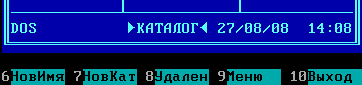
\includegraphics[width=0.5\textwidth]{patterns/01_helloworld/Norton_Commander_v5_51.png}
\caption{Русифицированный Norton Commander 5.51}
\end{figure}

Вероятно, так было и с другими языками в других странах.

\myindex{Borland Delphi}
В строках в Delphi, длина строки также должна быть поправлена, если нужно.


\subsection{x86-64}
\EN{\subsubsection{MSVC: x86-64}

\myindex{x86-64}
Let's also try 64-bit MSVC:

\lstinputlisting[caption=MSVC 2012 x64,style=customasmx86]{patterns/01_helloworld/MSVC_x64.asm}

\myindex{fastcall}

In x86-64, all registers were extended to 64-bit, and now their names have an \TT{R-} prefix.
In order to use the stack less often (in other words, to access external memory/cache less often), there is
a popular way to pass function arguments via registers (\emph{fastcall}) \myref{fastcall}.
I.e., a part of the function's arguments are passed in registers, and the rest---via the stack.
In Win64, 4 function arguments are passed in the \RCX, \RDX, \Reg{8}, and \Reg{9} registers.
That is what we see here: a pointer to the string for \printf is now passed not in the stack, but rather in the \RCX register.
The pointers are 64-bit now, so they are passed in the 64-bit registers (which have the \TT{R-} prefix).
However, for backward compatibility, it is still possible to access the 32-bit parts, using the \TT{E-} prefix.
This is how the \RAX/\EAX/\AX/\AL register looks like in x86-64:

\RegTableOne{RAX}{EAX}{AX}{AH}{AL}

The \main function returns an \Tint{}-typed value, which in \CCpp is still 32-bit, for better backward compatibility
and portability, so that is why the \EAX register is cleared at the function end (i.e., the 32-bit
part of the register) instead of with \RAX{}.
There are also 40 bytes allocated in the local stack.
This is called the \q{shadow space}, which we'll talk about later: \myref{shadow_space}.
}
\FR{\subsubsection{MSVC: x86-64}

\myindex{x86-64}
Essayons MSVC 64-bit:

\lstinputlisting[caption=MSVC 2012 x64,style=customasmx86]{patterns/01_helloworld/MSVC_x64.asm}

\myindex{fastcall}

En x86-64, tous les registres ont été étendus à 64-bit et leurs noms ont maintenant le préfixe \TT{R-}.
Afin d'utiliser la pile moins souvent (en d'autres termes, pour accéder moins souvent à la mémoire externe/au cache),
il existe un moyen répandu de passer les arguments aux fonctions par les registres (\emph{fastcall}) \myref{fastcall}.
I.e., une partie des arguments de la fonction est passée par les registres, le reste---par la pile.
En Win64, 4 arguments de fonction sont passés dans les registres \RCX, \RDX, \Reg{8}, \Reg{9}.
C'est ce que l'on voit ci-dessus: un pointeur sur la chaîne pour \printf est passé non pas par la pile,
mais par le registre \RCX.
Les pointeurs font maintenant 64-bit, ils sont donc passés dans les registres 64-bit (qui ont le préfixe \TT{R-}).
Toutefois, pour la rétrocompatibilité, il est toujours possible d'accéder à la partie 32-bits des registres,
en utilisant le préfixe \TT{E-}.
Voici à quoi ressemblent les registres \RAX/\EAX/\AX/\AL en x86-64:

\RegTableOne{RAX}{EAX}{AX}{AH}{AL}

La fonction \main renvoie un type \Tint{}, qui est, en \CCpp, pour une meilleure rétrocompatibilité
et portabilité, toujours 32-bit, c'est pourquoi le registre \EAX est mis à zéro à la fin de la fonction (i.e., la
partie 32-bit du registre) au lieu de \RAX{}.
Il y aussi 40 octets alloués sur la pile locale.
Cela est appelé le \q{shadow space}, dont nous parlerons plus tard: \myref{shadow_space}.
}
\IT{\subsubsection{MSVC: x86-64}

\myindex{x86-64}
Proviamo anche con MSVC a 64-bit:

\lstinputlisting[caption=MSVC 2012 x64,style=customasmx86]{patterns/01_helloworld/MSVC_x64.asm}

\myindex{fastcall}

In x86-64, tutti i registri sono stati estesi a 64-bit ed il loro nome ha il prefisso \TT{R-}.
Per usare lo stack meno spesso (in altre parole, per accedere meno spesso alla memoria esterna/cache), esiste un metodo molto diffuso per passare gli argomenti delle funzioni tramite i registri (\emph{fastcall}) \myref{fastcall}.
Ovvero, una parte degli argomenti viene passata attraverso i registri, il resto ---attraverso lo stack.
In Win64, 4 argomenti di funzione sono passati nei registri \RCX, \RDX, \Reg{8}, \Reg{9}.
Questo è ciò che vediamo qui: un puntatore alla stringa per \printf è adesso passato nel registro \RCX anziché tramite lo stack.
I puntatori adesso sono a 64-bit, quindi vengono passati nei registri a 64-bit (aventi il prefisso \TT{R-}).
E' comunque possibile, per retrocompatibilità, accedere alle parti a 32-bit, usando il prefisso \TT{E-}.
I registri \RAX/\EAX/\AX/\AL in x86-64 appaiono così:

\RegTableOne{RAX}{EAX}{AX}{AH}{AL}

La funzione \main restituisce un valore di tipo \Tint{}, che in \CCpp, per migliore retrocompatibilità e portabilità, resta ancora a 32-bit, motivo per cui il registro \EAX (quindi la parte a 32 bit del registro) viene svuotato invece di \RAX{} alla fine della funzione.
Ci sono anche 40 byte allocati nello stack locale.
Questo spazio è detto \q{shadow space}, e ne parleremo più avanti: \myref{shadow_space}.
}
\NL{\subsubsection{MSVC: x86-64}

\myindex{x86-64}
Laat ons ook eens kijken naar 64-bit MSVC:

\lstinputlisting[caption=MSVC 2012 x64,style=customasmx86]{patterns/01_helloworld/MSVC_x64.asm}

\myindex{fastcall}

In x86-64 zijn alle registers uitgebreid tot 64-bit, en hebben hun namen een \TT{R-} prefix gekregen.
Om de stack minder te gebruiken (met andere woorden, om het externe geheugen/cache minder vaak te benaderen), bestaat
er een populaire manier om functies parameters door te geven via registers (\emph{fastcall}) \myref{fastcall}.
Bv., een deel van de parameters wordt doorgegeven via het register, de rest --- via de stack.
In Win64, worden 4 functie parameters doorgegeven via de \RCX, \RDX, \Reg{8}, \Reg{9} registers.
Dat is wat we hier zien: een pointer naar de string voor \printf wordt doorgegeven, niet via de stack, maar via het \RCX register.
De pointers zijn 64-bit nu, dus worden ze doorgegeven in de 64-bit registers (dewelke de \TT{R-} prefix hebben).
Voor backward compatibility is het echter nog steeds mogelijk om de 32-bit gedeelten aan te spreken, door gebruik te maken van de \TT{E-} prefix.
Dit is hoe de \RAX/\EAX/\AX/\AL registers eruit zien in x86-64:

\RegTableOne{RAX}{EAX}{AX}{AH}{AL}

De \main functie geeft een \Tint{}-typed waarde terug, hetwelk, in \CCpp, voor betere backward compatibiliteit
en portabiliteit, nog steeds 32-bit is. Daarom wordt het \EAX register ook leeggemaakt bij het einde van de functie
(het 32-bit gedeelte van het register) in plaats van \RAX{}.
Er zijn ook 40 bytes gealloceerd op de lokale stack.
Dit wordt de \q{shadow space} genoemd, waarover we het later nog gaan hebben: \myref{shadow_space}.

}
\RU{\subsubsection{MSVC: x86-64}

\myindex{x86-64}
Попробуем также 64-битный MSVC:

\lstinputlisting[caption=MSVC 2012 x64,style=customasmx86]{patterns/01_helloworld/MSVC_x64.asm}

\myindex{fastcall}

В x86-64 все регистры были расширены до 64-х бит и теперь имеют префикс \TT{R-}.
Чтобы поменьше задействовать стек (иными словами, поменьше обращаться к кэшу и внешней памяти), уже давно имелся
довольно популярный метод передачи аргументов функции через регистры (\emph{fastcall}) \myref{fastcall}.
Т.е. часть аргументов функции передается через регистры и часть ---через стек.
В Win64 первые 4 аргумента функции передаются через регистры \RCX, \RDX, \Reg{8}, \Reg{9}.
Это мы здесь и видим: указатель на строку в \printf теперь передается не через стек, а через регистр \RCX.
Указатели теперь 64-битные, так что они передаются через 64-битные части регистров (имеющие префикс \TT{R-}).
Но для обратной совместимости можно обращаться и к нижним 32 битам регистров используя префикс \TT{E-}.
Вот как выглядит регистр \RAX/\EAX/\AX/\AL в x86-64:

\RegTableOne{RAX}{EAX}{AX}{AH}{AL}

Функция \main возвращает значение типа \Tint, который в \CCpp, надо полагать, для лучшей совместимости и переносимости,
оставили 32-битным. Вот почему в конце функции \main обнуляется не \RAX, а \EAX, т.е. 32-битная часть регистра.
Также видно, что 40 байт выделяются в локальном стеке.
Это \q{shadow space} которое мы будем рассматривать позже: \myref{shadow_space}.
}
\PTBR{\subsubsection{MSVC: x86-64}

\myindex{x86-64}
Vamos tentar também o MSVC 64-bits:

\lstinputlisting[caption=MSVC 2012 x64,style=customasmx86]{patterns/01_helloworld/MSVC_x64.asm}

\myindex{fastcall}

No x86-64, todos os registradores foram extendidos para 64-bits e agora seus nomes contém um \TT{R-} no prefixo.
A fim de diminuir a frequência com que a stack (pilha) é usada (em outras palavras, para acessar memória externa/cache menos vezes),
existe uma maneira popular de passar argumentos para funções através dos registradores (\emph{fastcall}) \myref{fastcall}.
Por exemplo, uma parte dos argumentos da função é passada nos registradores, o resto pela stack.
No Win64, 4 argumentos de funções são passados através dos registradores \RCX, \RDX, \Reg{8}, \Reg{9}.
Que é o que nós vemos, um ponteiro para a string para o printf() não é passado pela stack, mas no registrador \RCX.
Os ponteiros são 64-bits agora, então, eles são passados através dos registradores de 64-bits (que tem prefixo \TT{R-}).
Entretanto, para compatibilidade, ainda é possível acessar partes de 32-bits, usando o prefixo \TT{E-}.
É assim que os registradores \RAX/\EAX/\AX/\AL se parecem no x86-64:

\RegTableOne{RAX}{EAX}{AX}{AH}{AL}

A função \main retorna um valor do tipo inteiro, que em \CCpp é melhor para compatibilidade com versões anteriores e portabilidade,
de 32-bits, por isso o registrador \EAX é limpo no final da função (a parte de 32-bits do registrador) ao invés de \RAX.
Há também 40 bytes alocados na pilha local.
Que é chamado de ``shadow space'', o qual falaremos mais tarde: \myref{shadow_space}.

}
\DE{\subsubsection{MSVC: x86-64}

\myindex{x86-64}
Hier das gleiche Beispiel mit der 64-Bit-Variante von MSVC kompiliert:

\lstinputlisting[caption=MSVC 2012 x64,style=customasmx86]{patterns/01_helloworld/MSVC_x64.asm}

\myindex{fastcall}

In x86-64 wurden alle Regeister auf 64-Bit erweitert und die Registernamen mit einem \TT{R-}Prefix versehen.
Um den Stack weniger oft zu nutzen (also um auf externen Speicher / Cache selterner zuzugreifen), existiert
ein verbreiteter Weg um Funktionsargumente per Register (\emph{fastcall}) \myref{fastcall} zu übergeben.
Das heißt ein Teil der Funktionsargumente wird in Registern übergeben, der Rest---über den Stack.
In Win64 werden vier Funktionsargumente in den Registern \RCX, \RDX, \Reg{8} und \Reg{9} übergeben.
Das ist was hier sichtbar ist: der Zeiger zu der Zeichenkette für \printf ist jetzt nicht im Stack übergeben sondern im \RCX-Register.
Die Zeiger sind nun 64-Bit breit, also werden sie in den 64-Bit-Registern übergeben (die jetz den \TT{R-}Prefix haben).
Aus Gründen der Rückwärtskompatibilität ist es aber immer noch möglich mit dem \TT{E-}Prefix auf 32-Bit-Teile zuzugrifen.
Nachfolgend, der Aufbau der \RAX/\EAX/\AX/\AL-Register in x86-64:

\RegTableOne{RAX}{EAX}{AX}{AH}{AL}

Die \main-Funktion gibt einen Wert vom Typ \Tint{} zurück, der in \CCpp aus Gründen der Kompatibilität und
Portabilität immernoch 32 Bit breit ist. Daher wird am Ende der Funktion das \EAX-Register auf Null gesetzt
(das heißt der 32-Bit-Part des Registers) anstatt \RAX{}.
Auf dem lokalen Stack sind zusätzliche 40 Byte reserviert.
Dieser Bereich wird \q{shadow space} genannt und wird in Abschnitt \myref{shadow_space} noch genauer betrachtet.
}
\PL{\subsubsection{MSVC: x86-64}

\myindex{x86-64}
Przyjrzyjmy się wynikom kompilacji 64-bitowego MSVC:

\lstinputlisting[caption=MSVC 2012 x64,style=customasmx86]{patterns/01_helloworld/MSVC_x64.asm}

\myindex{fastcall}

W x86-64 wszystkie rejestry zostały rozszerzone do 64 bitów i ich nazwy zyskały prefiks \TT{R-}.
Żeby jak najrzadziej korzystać ze stosu (inaczej mówiąc, jak najmniej korzystać z pamięci cache i pamięci zewnętrznej), istnieje popularna metoda przekazywania argumentów funkcji przez rejestry (\emph{fastcall}) \myref{fastcall}.
Tzn. część argumentów funkcji jest przekazywana przez rejestry a część --- przez stos.
W Win64 pierwsze 4 argumenty funkcji są przekazywane przez rejestry \RCX, \RDX, \Reg{8} i \Reg{9}.
Widać to w powyższym przykładzie: wskaźnik na argument funkcji \printf (łańcuch znaków) teraz jest przekazywany nie przez stos, a przez rejestr \RCX.
Wskaźniki są teraz 64-bitowe, więc są przekazywane przez przez 64-bitowe rejestry (mające prefiks \TT{R-}).
Ale dla wstecznej kompatybilności można adresować również młodsze 32 bity rejestrów poprzez prefiks \TT{E-}.
W ten oto sposób wygląda rejestr \RAX/\EAX/\AX/\AL w x86-64:

\RegTableOne{RAX}{EAX}{AX}{AH}{AL}

Funkcja \main zwraca wartość typu \Tint, który w \CCpp, dla większej kompatybilności,
pozostał 32-bitowy. Właśnie dlatego na końcu funkcji \main zeruje się nie \RAX, a \EAX, czyli 32-bitową część rejestru.
Dodatkowo na stosie lokalnym jest zarezerwowanych 40 bajtów.
Jest to tzw. \q{shadow space}, który będzie omawiany później: \myref{shadow_space}.

}
\JA{\subsubsection{MSVC: x86-64}

\myindex{x86-64}
64ビットのMSVCも試してみましょう。

\lstinputlisting[caption=MSVC 2012 x64,style=customasmx86]{patterns/01_helloworld/MSVC_x64.asm}

\myindex{fastcall}

x86-64では、すべてのレジスタが64ビットに拡張されましたが、その名前には\TT{R-}プレフィックスが付いています。 
スタックをあまり頻繁に使用しないように(言い換えると、外部メモリ/キャッシュにアクセスする頻度を減らす)、
レジスタ(\emph{fastcall}) \myref{fastcall}を介して関数引数を渡す一般的な方法があります。 
すなわち、関数の引数の一部はレジスタに渡され、残りはスタックに渡されます。 
Win64では、4つの関数引数が \RCX 、 \RDX 、 \Reg{8} 、および \Reg{9} レジスタに渡されます。 
ここで見るものは: \printf の文字列へのポインタはスタックにではなく、 \RCX レジスタに渡されます。 
ポインタは現在64ビットであるため、64ビットレジスタ(\TT{R-}プレフィックスを持つ)に渡されます。 
ただし、下位互換性を保つために、\TT{E-}接頭辞を使用して32ビットのパーツにアクセスすることは可能です。 
これは、 \RAX/\EAX/\AX/\AL レジスタがx86-64のように見える方法です。

\RegTableOne{RAX}{EAX}{AX}{AH}{AL}

\main 関数は\Tint{}型の値を返します。これは \CCpp では32ビットのままで、下位互換性と移植性を向上させるため、
関数終了時に \RAX レジスタの代わりに \EAX レジスタがクリアされる理由です。(すなわちレジスタの32ビットの部分) 
ローカルスタックには40バイトも割り当てられています。 
これは\q{シャドースペース}と呼ばれます。これについては後で説明します:\myref{shadow_space}
}

\EN{\subsubsection{GCC: x86-64}

\myindex{x86-64}
Let's also try GCC in 64-bit Linux:

\lstinputlisting[caption=GCC 4.4.6 x64,style=customasmx86]{patterns/01_helloworld/GCC_x64_EN.s}

% I think I got the intent right on the following line - Renaissance
Linux, *BSD and \MacOSX also use a method to pass function arguments in registers. \SysVABI{}.

The first 6 arguments are passed in the \RDI, \RSI, \RDX, \RCX, \Reg{8}, and \Reg{9}  registers, and the rest---via the stack.

So the pointer to the string is passed in \EDI (the 32-bit part of the register).
Why doesn't it use the 64-bit part, \RDI?

It is important to keep in mind that all \MOV instructions in 64-bit mode that write something into the lower 32-bit register part also clear the higher 32-bits (as stated in Intel manuals: \myref{x86_manuals}).\\
I.e., the \INS{MOV EAX, 011223344h} writes a value into \RAX correctly, since the higher bits will be cleared.

If we open the compiled object file (.o), we can also see all the instructions' opcodes
\footnote{This must be enabled in \textbf{Options $\rightarrow$ Disassembly $\rightarrow$ Number of opcode bytes}}:

\lstinputlisting[caption=GCC 4.4.6 x64,style=customasmx86]{patterns/01_helloworld/GCC_x64.lst}

\label{hw_EDI_instead_of_RDI}
As we can see, the instruction that writes into \EDI at \TT{0x4004D4} occupies 5 bytes.
The same instruction writing a 64-bit value into \RDI occupies 7 bytes.
Apparently, GCC is trying to save some space.
Besides, it can be sure that the data segment containing the string will not be allocated at the addresses higher than 4\gls{GiB}.

\label{SysVABI_input_EAX}
% There isn't an ABI acronym in acronyms.tex - I figure the intent is to Application Binary Interface,
% so I put it in there (in the EN section, commented out)
We also see that the \EAX register has been cleared before the \printf function call.
This is done because according to \ac{ABI} standard mentioned above,
the number of used vector registers is to be passed in \EAX in *NIX systems on x86-64.
}
\FR{\subsubsection{GCC: x86-64}

\myindex{x86-64}
Essayons GCC sur un Linux 64-bit:

\lstinputlisting[caption=GCC 4.4.6 x64,style=customasmx86]{patterns/01_helloworld/GCC_x64_FR.s}

Une méthode de passage des arguments à la fonction dans des registres est aussi utilisée sur Linux, *BSD et
\MacOSX est \SysVABI.
Linux, *BSD et \MacOSX utilisent aussi une méthode pour passer les arguments d'une
fonction par les registres: \SysVABI{}.

Les 6 premiers arguments sont passés dans les registres \RDI, \RSI, \RDX, \RCX, \Reg{8}, \Reg{9} et les autres---par
la pile.

Donc le pointeur sur la chaîne est passé dans \EDI (la partie 32-bit du registre).
Mais pourquoi ne pas utiliser la partie 64-bit, \RDI?

Il est important de garder à l'esprit que toutes les instructions \MOV en mode 64-bit qui écrivent quelque chose
dans la partie 32-bit inférieuaer du registre efface également les 32-bit supérieurs (comme indiqué dans les manuels Intel:
\myref{x86_manuals}).\\
I.e., l'instruction \INS{MOV EAX, 011223344h} écrit correctement une valeur dans \RAX, puisque que les bits supérieurs
sont mis à zéro.

Si nous ouvrons le fichier objet compilé (.o), nous pouvons voir tous les opcodes des instructions
\footnote{Ceci doit être activé dans \textbf{Options $\rightarrow$ Disassembly $\rightarrow$ Number of opcode bytes}}:

\lstinputlisting[caption=GCC 4.4.6 x64,style=customasmx86]{patterns/01_helloworld/GCC_x64.lst}

\label{hw_EDI_instead_of_RDI}
Comme on le voit, l'instruction qui écrit dans \EDI en \TT{0x4004D4} occupe 5 octets.
La même instruction qui écrit une valeur sur 64-bit dans \RDI occupe 7 octets.
Il semble que GCC essaye d'économiser un peu d'espace.
En outre, cela permet d'être sûr que le segment de données contenant la chaîne ne sera pas alloué à une adresse supérieure
à 4 \gls{GiB}.

\label{SysVABI_input_EAX}
Nous voyons aussi que le registre \EAX est mis à zéro avant l'appel à la fonction \printf.
Ceci, car conformément à l'\ac{ABI} standard mentionnée plus haut,
le nombre de registres vectoriel utilisés est passé dans \EAX sur les systèmes *NIX en x86-64.

}
\RU{\subsubsection{GCC: x86-64}

\myindex{x86-64}
Попробуем GCC в 64-битном Linux:

\lstinputlisting[caption=GCC 4.4.6 x64,style=customasmx86]{patterns/01_helloworld/GCC_x64_RU.s}

В Linux, *BSD и \MacOSX для x86-64 также принят способ передачи аргументов функции через регистры \SysVABI.

6 первых аргументов передаются через регистры \RDI, \RSI, \RDX, \RCX, \Reg{8}, \Reg{9}, а остальные --- через стек.

Так что указатель на строку передается через \EDI (32-битную часть регистра).
Но почему не через 64-битную часть, \RDI?

Важно запомнить, что в 64-битном режиме все инструкции \MOV, записывающие что-либо в младшую 32-битную часть регистра, обнуляют старшие 32-бита (это можно найти в документации от Intel: \myref{x86_manuals}).
То есть, инструкция \INS{MOV EAX, 011223344h} корректно запишет это значение в \RAX, старшие биты сбросятся в ноль.

Если посмотреть в \IDA скомпилированный объектный файл (.o), увидим также опкоды всех инструкций
\footnote{Это нужно задать в \textbf{Options $\rightarrow$ Disassembly $\rightarrow$ Number of opcode bytes}}:

\lstinputlisting[caption=GCC 4.4.6 x64,style=customasmx86]{patterns/01_helloworld/GCC_x64.lst}

\label{hw_EDI_instead_of_RDI}
Как видно, инструкция, записывающая в \EDI по адресу \TT{0x4004D4}, занимает 5 байт.
Та же инструкция, записывающая 64-битное значение в \RDI, занимает 7 байт.
Возможно, GCC решил немного сэкономить.
К тому же, вероятно, он уверен, что сегмент данных, где хранится строка, никогда не будет расположен в адресах выше 4\gls{GiB}.

\label{SysVABI_input_EAX}
Здесь мы также видим обнуление регистра \EAX перед вызовом \printf.
Это делается потому что по упомянутому выше стандарту передачи аргументов в *NIX для x86-64 в \EAX передается количество задействованных векторных регистров.

}
\NL{\subsubsection{GCC: x86-64}

\myindex{x86-64}
Laat ons ook eens kijken naar GCC in 64-bit Linux:

% TODO translate:
\lstinputlisting[caption=GCC 4.4.6 x64,style=customasmx86]{patterns/01_helloworld/GCC_x64_EN.s}

Een methode om functieargumenten door te geven in registers wordt ook gebruikt in Linux, *BSD en \MacOSX \SysVABI.

De eerste 6 argumenten worden doorgegeven in de \RDI, \RSI, \RDX, \RCX, \Reg{8}, \Reg{9} registers, en de rest --- via de stack.

De pointer naar de string wordt dus doorgegeven via \EDI (het 32-bit gedeelte van het register).
Maar waarom gebruikt men niet het 64-bit gedeelte, \RDI?

Het is belangrijk te onthouden dat alle \MOV instructies in 64-bit modus, die iets schrijven in het onderste 32-bit gedeelte van het register, ook het bovenste 32-bit gedeelte leegmaken.
\INS{MOV EAX, 011223344h} schrijft een waarde correct weg in \RAX, aangezien de bovenste bits zullen worden leeggemaakt.

Als we het gecompileerde object-bestand (.o) openen, kunnen we ook de opcodes zien van alle instructies
\footnote{Dit moet ook geactiveerd worden in \textbf{Options $\rightarrow$ Disassembly $\rightarrow$ Number of opcode bytes}}:

\lstinputlisting[caption=GCC 4.4.6 x64,style=customasmx86]{patterns/01_helloworld/GCC_x64.lst}

\label{hw_EDI_instead_of_RDI}
Zoals je kan zien, bezet de instructie die in \EDI schrijft op \TT{0x4004D4} 5 bytes.
Dezelfde instructie die een 64-bit waarde in \RDI schrijft, bezet 7 bytes.
Blijkbaar probeert GCC wat plaats te besparen.
Daarnaast kunnen we met zekerheid zeggen dat het data segment dat de string bevat, niet zal gealloceerd worden op de adressen hoger dan 4\gls{GiB}.

\label{SysVABI_input_EAX}
We zien ook dat het \EAX register leeggemaakt is voor de \printf functie call.
Dit wordt gedaan omdat het aantal gebruikte vector registers wordt doorgegeven in \EAX in *NIX systemen op x86-64.

}
\IT{\subsubsection{GCC: x86-64}

\myindex{x86-64}
Proviamo anche GCC in Linux a 64-bit:

\lstinputlisting[caption=GCC 4.4.6 x64,,style=customasmx86]{patterns/01_helloworld/GCC_x64_IT.s}

% I think I got the intent right on the following line - Renaissance
Linux, *BSD e \MacOSX usano anche un metodo per passare argomenti di funzione nei registri. \SysVABI.

I primi 6 argomenti sono passati nei registri \RDI, \RSI, \RDX, \RCX, \Reg{8}, \Reg{9}, ed il resto---tramite lo stack.

Quindi il puntatore alla stringa viene passato in \EDI (la parte a 32-bit del registro).
Ma perchè non utilizza la parte a 64-bit, \RDI?

E' importante ricordare che tutte le istruzioni \MOV in modalità 64-bit che scrivono qualcosa nella parte dei 32-bit bassa di un registro, azzera anche la parte a 32-bit alta (come indicato nei manuali Intel: \myref{x86_manuals}).\\
Ad esempio, \INS{MOV EAX, 011223344h} scrive correttamente un valore in \RAX, poichè i bit della parte alta verranno azzerati.

Se apriamo il file oggetto compilato (.o), possiamo anche vedere gli opcode di tutte le istruzioni
\footnote{Questo deve essere abilitato in \textbf{Options $\rightarrow$ Disassembly $\rightarrow$ Number of opcode bytes}}:

\lstinputlisting[caption=GCC 4.4.6 x64,style=customasmx86]{patterns/01_helloworld/GCC_x64.lst}

\label{hw_EDI_instead_of_RDI}
Come possiamo notare, l'istruzione che scrive in \EDI all'indirizzo \TT{0x4004D4} occupa 5 byte.
La stessa istruzione che scrive un valore a 64-bit in \RDI occupa 7 bytes.
Apparentemente, GCC sta cercando di risparmiare un po' di spazio.
Inoltre, può essere sicuro che il segmento dati contenente la stringa non sarà allocato ad indirizzi maggiori di 4\gls{GiB}.

\label{SysVABI_input_EAX}
% There isn't an ABI acronym in acronyms.tex - I figure the intent is to Application Binary Interface,
% so I put it in there (in the EN section, commented out)
Notiamo anche che il registro \EAX è stato azzerato prima della chiamata alla funzione \printf.
Questo viene fatto perché, in base allo standard \ac{ABI} citato in precedenza,
il numero dei registri vettore usati deve essere passato in \EAX nei sistemi *NIX su x86-64.
}
\DE{\subsubsection{GCC: x86-64}

\myindex{x86-64}
Nachfolgend das Beispiel unter einem 64 Bit-Linux-System mit GCC kompoliert:

\lstinputlisting[caption=GCC 4.4.6 x64,style=customasmx86]{patterns/01_helloworld/GCC_x64_DE.s}

Eine Methode im Funktionsargumente in Registern zu übergeben, wird auch in Linux, *BSD und \MacOSX genutzt und heißt \SysVABI.

Die ersten sechs Argumente sind in den Registern \RDI, \RSI, \RDX, \RCX,\Reg{8} und \Reg{9} übergeben und der Rest---über den Stack.

Der Zeiger zu der Zeichenkette ist in \EDI (also, dem 32-Bit-Teil) gesichert.
Warum wird nicht der 64-Bit-Teil \RDI genutz?

Es ist wichtig sich zu vergegenwertigen, dass alle \MOV-Anweisungen im 64-Bit-Modus, die etwas in den niederwertigen 32-Bit-Teil eines Registers schreiben,
auch den höherwertigen 32-Bit-Teil des Registers löschen (siehe Intel-Handbücher: \myref{x86_manuals}).\\
Die Anweisung \INS{MOV EAX, 011223344h} schreibt also den richtigen Wert in \RAX, weil die höherwetigen Bits auf Null gesetzt werden.

In der Objekt-Datei (.o) eines Kompilats sind ebenfalls alles OpCodes der verwendeten Anweisungen zu sehen.
\footnote{Dies muss aktiviert werden: \textbf{Optionen $\rightarrow$ Disassembly $\rightarrow$ Number of opcode bytes}}:

\lstinputlisting[caption=GCC 4.4.6 x64,style=customasmx86]{patterns/01_helloworld/GCC_x64.lst}

\label{hw_EDI_instead_of_RDI}
Wie man sehen kann verändert die Anweisung zum Schreiben in \EDI an der Adresse \TT{0x4004D4} fünf Byte.
Dieselbe Anweisung die einen 64-Bit-Wert in \RDI schreibt, verändert 7 Bytes.
Offenstichtlich versucht GCC etwas Speicherplatz zu sparen.
Nebenbei ist es sicher, dass das Datensegment, welches die Zeichenkette entählt niemals an Adressen höher 4\gls{GiB} reserviert wird.

\label{SysVABI_input_EAX}
Es ist auch erkennbar, dass das \EAX-Register vor dem Aufruf von \printf zurückgesetzt wurde.
Dies geschieht, aufgrund der Konvention in der oben genannten \ac{ABI}, dass in *NIX-Systemen auf x86-64-Architektur
die Anzahl der genutzten Vektor-Register in \EAX übergeben wird.
}
\PL{\subsubsection{GCC: x86-64}

\myindex{x86-64}
Przyjrzyjmy się wynikom kompilacji GCC na 64-bitowym systemie Linux:

\lstinputlisting[caption=GCC 4.4.6 x64,style=customasmx86]{patterns/01_helloworld/GCC_x64_PL.s}

Na Linuksie, *BSD i \MacOSX w architekturze x86-64 argumenty funkcji także przekazuje się przez rejestry \SysVABI.

6 pierwszych argumentów jest przekazywanych przez rejestry \RDI, \RSI, \RDX, \RCX, \Reg{8} i \Reg{9}, a reszta --- przez stos.

Wskaźnik na łańcuch znaków jest przekazywany przez \EDI (32-bitową część rejestru). Dlaczego nie użyto 64-bitowego \RDI?

Warto pamiętać, że w 64-bitowym trybie wszystkie instrukcje \MOV, zapisujące cokolwiek do młodszej 32-bitowej części rejestru, zerują starsze 32 bity (jest to opisane w dokumentacji Intela: \myref{x86_manuals}).
Z tego powodu instrukcja \INS{MOV EAX, 011223344h} poprawnie zapisze tę wartość do \RAX, a starsze bity się wyzerują.

Jeślibyśmy podejrzeli w deasemblerze \IDA skompilowany plik (.o), to zobaczylibyśmy kody operacji (opcode) wszystkich instrukcji
\footnote{Trzeba włączyć tę opcję w \textbf{Options $\rightarrow$ Disassembly $\rightarrow$ Number of opcode bytes}}:

\lstinputlisting[caption=GCC 4.4.6 x64,style=customasmx86]{patterns/01_helloworld/GCC_x64.lst}

\label{hw_EDI_instead_of_RDI}
Jak widać, instrukcja \MOV pod adresem \TT{0x4004D4}, która zapisuje do \EDI, zajmuje 5 bajtów.
Ta sama instrukcja, zapisująca 64-bitową wartość do \RDI, zajmuje 7 bajtów.
Najwyraźniej GCC stara się zaoszczędzić trochę miejsca.
GCC jest również pewne, że segment danych, w którym przechowywany jest łańcuch znaków, nigdy nie będzie zaalokowany pod adresem powyżej 4\gls{GiB}.

\label{SysVABI_input_EAX}
Widać również, że rejestr \EAX został wyzerowany przed wywołaniem funkcji \printf.
Zgodnie ze standardem \ac{ABI} opisanym wyżej, w *NIX dla x86-64 w \EAX jest ustawiana liczba użytych rejestrów wektorowych do przekazania argumentów zmiennoprzecinkowych, jeśli funkcja może przyjmować zmienną liczbę argumentów.
Nie został wykorzystany żaden taki rejestr, a \printf jest funkcją o zmiennej liczbie argumentów, więc należy ustawić \EAX na 0.
}
\JA{\subsubsection{GCC: x86-64}

\myindex{x86-64}
64ビット環境のLinuxでGCCを試してみましょう。

\lstinputlisting[caption=GCC 4.4.6 x64,style=customasmx86]{patterns/01_helloworld/GCC_x64_JA.s}

% I think I got the intent right on the following line - Renaissance
Linux、*BSDと \MacOSX は関数引数をレジスタに渡すためのメソッドも使います: \SysVABI{}

最初の6つの引数は、\RDI, \RSI, \RDX, \RCX, \Reg{8} および \Reg{9}レジスタに渡され、残りはスタックを介して渡されます。

そのため、文字列へのポインタは \EDI (レジスタの32ビット部分)に渡されます。 なぜ64ビット版の \RDI を使用しないのでしょうか。

下位の32ビットレジスタ部分に何かを書き込む64ビットモードのすべての \MOV 命令も上位32ビットをクリアすることが重要です(インテルマニュアル:\myref{x86_manuals}を参照)。 つまり、\INS{MOV EAX, 011223344h}は、上位ビットがクリアされるため、 \RAX に値を正しく書き込みます。

コンパイルされたオブジェクトファイル(.o)を開くと、すべての命令のオペコードも見ることができます。
\footnote{これは \textbf{オプション $\rightarrow$ ディスアセンブル $\rightarrow$ オペコードバイト数} で有効になるはずです}:

\lstinputlisting[caption=GCC 4.4.6 x64,style=customasmx86]{patterns/01_helloworld/GCC_x64.lst}

\label{hw_EDI_instead_of_RDI}
ご覧のように、\TT{0x4004D4}の \EDI に書き込む命令は5バイトを占有します。 
64ビット値を \RDI に書き込む同じ命令は7バイトを占有します。 
明らかに、GCCはいくらかのスペースを節約しようとしています。 
さらに、文字列を含むデータセグメントが4\gls{GiB}以上のアドレスに割り当てられないことが保証されます。

\label{SysVABI_input_EAX}
% There isn't an ABI acronym in acronyms.tex - I figure the intent is to Application Binary Interface,
% so I put it in there (in the EN section, commented out)
また、 \printf 関数呼び出しの前に \EAX レジスタがクリアされていることがわかります。 
上記の\ac{ABI}標準によれば、使用されたベクトルレジスタの数はx86-64の*NIXシステムで \EAX に渡されるためです。
}

\subsubsection{Коррекция (патчинг) адреса (Win64)}

Если наш пример скомпилирован в MSVC 2013 используя опцию \TT{/MD}
(подразумевая меньший исполняемый файл из-за внешнего связывания файла \TT{MSVCR*.DLL}),
ф-ция \main идет первой, и её легко найти:

\begin{figure}[H]
\centering
\myincludegraphics{patterns/01_helloworld/hiew_incr1.png}
\caption{Hiew}
\label{}
\end{figure}

В качестве эксперимента, мы можем \glslink{increment}{инкрементировать} адрес на 1:

\begin{figure}[H]
\centering
\myincludegraphics{patterns/01_helloworld/hiew_incr2.png}
\caption{Hiew}
\label{}
\end{figure}

Hiew показывает строку \q{ello, world}.
И когда мы запускаем исполняемый файл, именно эта строка и выводится.

\subsubsection{Выбор другой строки из исполняемого файла (Linux x64)}

Исполняемый файл, если скомпилировать используя GCC 5.4.0 на Linux x64, имеет множество других строк:
в основном, это имена импортированных ф-ций и имена библиотек.

Запускаю objdump, чтобы посмотреть содержимое всех секций скомпилированного файла:

\begin{lstlisting}
% objdump -s a.out

a.out:     file format elf64-x86-64

Contents of section .interp:
 400238 2f6c6962 36342f6c 642d6c69 6e75782d  /lib64/ld-linux-
 400248 7838362d 36342e73 6f2e3200           x86-64.so.2.
Contents of section .note.ABI-tag:
 400254 04000000 10000000 01000000 474e5500  ............GNU.
 400264 00000000 02000000 06000000 20000000  ............ ...
Contents of section .note.gnu.build-id:
 400274 04000000 14000000 03000000 474e5500  ............GNU.
 400284 fe461178 5bb710b4 bbf2aca8 5ec1ec10  .F.x[.......^...
 400294 cf3f7ae4                             .?z.

...
\end{lstlisting}

Не проблема передать адрес текстовой строки \q{/lib64/ld-linux-x86-64.so.2} в вызов \TT{printf()}:

\begin{lstlisting}[style=customc]
#include <stdio.h>

int main()
{
    printf(0x400238);
    return 0;
}
\end{lstlisting}

Трудно поверить, но этот код печатает вышеуказанную строку.

Измените адрес на \TT{0x400260}, и напечатается строка \q{GNU}.
Адрес точен для конкретной версии GCC, GNU toolset, итд.
На вашей системе, исполняемый файл может быть немного другой, и все адреса тоже будут другими.
Также, добавление/удаление кода из исходных кодов, скорее всего, сдвинет все адреса вперед или назад.



\EN{\mysection{Task manager practical joke (Windows Vista)}
\myindex{Windows!Windows Vista}

Let's see if it's possible to hack Task Manager slightly so it would detect more \ac{CPU} cores.

\myindex{Windows!NTAPI}

Let us first think, how does the Task Manager know the number of cores?

There is the \TT{GetSystemInfo()} win32 function present in win32 userspace which can tell us this.
But it's not imported in \TT{taskmgr.exe}.

There is, however, another one in \gls{NTAPI}, \TT{NtQuerySystemInformation()}, 
which is used in \TT{taskmgr.exe} in several places.

To get the number of cores, one has to call this function with the \TT{SystemBasicInformation} constant
as a first argument (which is zero
\footnote{\href{http://msdn.microsoft.com/en-us/library/windows/desktop/ms724509(v=vs.85).aspx}{MSDN}}).

The second argument has to point to the buffer which is getting all the information.

So we have to find all calls to the \\
\TT{NtQuerySystemInformation(0, ?, ?, ?)} function.
Let's open \TT{taskmgr.exe} in IDA. 
\myindex{Windows!PDB}

What is always good about Microsoft executables is that IDA can download the corresponding \gls{PDB} 
file for this executable and show all function names.

It is visible that Task Manager is written in \Cpp and some of the function names and classes are really 
speaking for themselves.
There are classes CAdapter, CNetPage, CPerfPage, CProcInfo, CProcPage, CSvcPage, 
CTaskPage, CUserPage.

Apparently, each class corresponds to each tab in Task Manager.

Let's visit each call and add comment with the value which is passed as the first function argument.
We will write \q{not zero} at some places, because the value there was clearly not zero, 
but something really different (more about this in the second part of this chapter).

And we are looking for zero passed as argument, after all.

\begin{figure}[H]
\centering
\myincludegraphics{examples/taskmgr/IDA_xrefs.png}
\caption{IDA: cross references to NtQuerySystemInformation()}
\end{figure}

Yes, the names are really speaking for themselves.

When we closely investigate each place where\\
\TT{NtQuerySystemInformation(0, ?, ?, ?)} is called,
we quickly find what we need in the \TT{InitPerfInfo()} function:

\lstinputlisting[caption=taskmgr.exe (Windows Vista),style=customasmx86]{examples/taskmgr/taskmgr.lst}

\TT{g\_cProcessors} is a global variable, and this name has been assigned by 
IDA according to the \gls{PDB} loaded from Microsoft's symbol server.

The byte is taken from \TT{var\_C20}. 
And \TT{var\_C58} is passed to\\
\TT{NtQuerySystemInformation()} 
as a pointer to the receiving buffer.
The difference between 0xC20 and 0xC58 is 0x38 (56).

Let's take a look at format of the return structure, which we can find in MSDN:

\begin{lstlisting}[style=customc]
typedef struct _SYSTEM_BASIC_INFORMATION {
    BYTE Reserved1[24];
    PVOID Reserved2[4];
    CCHAR NumberOfProcessors;
} SYSTEM_BASIC_INFORMATION;
\end{lstlisting}

This is a x64 system, so each PVOID takes 8 bytes.

All \emph{reserved} fields in the structure take $24+4*8=56$ bytes.

Oh yes, this implies that \TT{var\_C20} is the local stack is exactly the
\TT{NumberOfProcessors} field of the \TT{SYSTEM\_BASIC\_INFORMATION} structure.

Let's check our guess.
Copy \TT{taskmgr.exe} from \TT{C:\textbackslash{}Windows\textbackslash{}System32} 
to some other folder 
(so the \emph{Windows Resource Protection} 
will not try to restore the patched \TT{taskmgr.exe}).

Let's open it in Hiew and find the place:

\begin{figure}[H]
\centering
\myincludegraphics{examples/taskmgr/hiew2.png}
\caption{Hiew: find the place to be patched}
\end{figure}

Let's replace the \TT{MOVZX} instruction with ours.
Let's pretend we've got 64 CPU cores.

Add one additional \ac{NOP} (because our instruction is shorter than the original one):

\begin{figure}[H]
\centering
\myincludegraphics{examples/taskmgr/hiew1.png}
\caption{Hiew: patch it}
\end{figure}

And it works!
Of course, the data in the graphs is not correct.

At times, Task Manager even shows an overall CPU load of more than 100\%.

\begin{figure}[H]
\centering
\myincludegraphics{examples/taskmgr/taskmgr_64cpu_crop.png}
\caption{Fooled Windows Task Manager}
\end{figure}

The biggest number Task Manager does not crash with is 64.

Apparently, Task Manager in Windows Vista was not tested on computers with a large number of cores.

So there are probably some static data structure(s) inside it limited to 64 cores.

\subsection{Using LEA to load values}
\label{TaskMgr_LEA}

Sometimes, \TT{LEA} is used in \TT{taskmgr.exe} instead of \TT{MOV} to set the first argument of \\
\TT{NtQuerySystemInformation()}:

\lstinputlisting[caption=taskmgr.exe (Windows Vista),style=customasmx86]{examples/taskmgr/taskmgr2.lst}

\myindex{x86!\Instructions!LEA}

Perhaps \ac{MSVC} did so because machine code of \INS{LEA} is shorter than \INS{MOV REG, 5} (would be 5 instead of 4).

\INS{LEA} with offset in $-128..127$ range (offset will occupy 1 byte in opcode) with 32-bit registers is even shorter (for lack of REX prefix)---3 bytes.

Another example of such thing is: \myref{using_MOV_and_pack_of_LEA_to_load_values}.
}%
\RU{\subsection{Обменять входные значения друг с другом}

Вот так:

\lstinputlisting[style=customc]{patterns/061_pointers/swap/5_RU.c}

Как видим, байты загружаются в младшие 8-битные части регистров \TT{ECX} и \TT{EBX} используя \INS{MOVZX}
(так что старшие части регистров очищаются), затем байты записываются назад в другом порядке.

\lstinputlisting[style=customasmx86,caption=Optimizing GCC 5.4]{patterns/061_pointers/swap/5_GCC_O3_x86.s}

Адреса обоих байтов берутся из аргументов и во время исполнения ф-ции находятся в регистрах \TT{EDX} и \TT{EAX}.

Так что исопльзуем указатели --- вероятно, без них нет способа решить эту задачу лучше.

}%
\FR{\subsection{Exemple \#2: SCO OpenServer}

\label{examples_SCO}
\myindex{SCO OpenServer}
Un ancien logiciel pour SCO OpenServer de 1997 développé par une société qui a disparue
depuis longtemps.

Il y a un driver de dongle special à installer dans le système, qui contient les
chaînes de texte suivantes:
\q{Copyright 1989, Rainbow Technologies, Inc., Irvine, CA}
et
\q{Sentinel Integrated Driver Ver. 3.0 }.

Après l'installation du driver dans SCO OpenServer, ces fichiers apparaissent dans
l'arborescence /dev:

\begin{lstlisting}
/dev/rbsl8
/dev/rbsl9
/dev/rbsl10
\end{lstlisting}

Le programme renvoie une erreur lorsque le dongle n'est pas connecté, mais le message
d'erreur n'est pas trouvé dans les exécutables.

\myindex{COFF}

Grâce à \ac{IDA}, il est facile de charger l'exécutable COFF utilisé dans SCO OpenServer.

Essayons de trouver la chaîne \q{rbsl} et en effet, elle se trouve dans ce morceau
de code:

\lstinputlisting[style=customasmx86]{examples/dongles/2/1.lst}

Oui, en effet, le programme doit communiquer d'une façon ou d'une autre avec le driver.

\myindex{thunk-functions}
Le seul endroit où la fonction \TT{SSQC()} est appelée est dans la \glslink{thunk
 function}{fonction thunk}:

\lstinputlisting[style=customasmx86]{examples/dongles/2/2.lst}

SSQ() peut être appelé depuis au moins 2 fonctions.

L'une d'entre elles est:

\lstinputlisting[style=customasmx86]{examples/dongles/2/check1_EN.lst}

\q{\TT{3C}} et \q{\TT{3E}} semblent familiers: il y avait un dongle Sentinel Pro de
Rainbow sans mémoire, fournissant seulement une fonction de crypto-hachage secrète.

Vous pouvez lire une courte description de la fonction de hachage dont il s'agit
ici: \myref{hash_func}.

Mais retournons au programme.

Donc le programme peut seulement tester si un dongle est connecté ou s'il est absent.

Aucune autre information ne peut être écrite dans un tel dongle, puisqu'il n'a pas
de mémoire.
Les codes sur deux caractères sont des commandes (nous pouvons voir comment les commandes
sont traitées dans la fonction \TT{SSQC()}) et toutes les autres chaînes sont hachées
dans le dongle, transformées en un nombre 16-bit.
L'algorithme était secret, donc il n'était pas possible d'écrire un driver de remplacement
ou de refaire un dongle matériel qui l'émulerait parfaitement.

Toutefois, il est toujours possible d'intercepter tous les accès au dongle et de
trouver les constantes auxquelles les résultats de la fonction de hachage sont comparées.

Mais nous devons dire qu'il est possible de construire un schéma de logiciel de protection
de copie robuste basé sur une fonction secrète de hachage cryptographique: il suffit
qu'elle chiffre/déchiffre les fichiers de données utilisés par votre logiciel.

Mais retournons au code:

Les codes 51/52/53 sont utilisés pour choisir le port imprimante LPT.
3x/4x sont utilisés pour le choix de la \q{famille} (c'est ainsi que les dongles
Sentinel Pro sont différenciés les uns des autres: plus d'un dongle peut être connecté
sur un port LPT).

La seule chaîne passée à la fonction qui ne fasse pas 2 caractères est "0123456789".

Ensuite, le résultat est comparé à l'ensemble des résultats valides.

Si il est correct, 0xC ou 0xB est écrit dans la variable globale \TT{ctl\_model}.%

Une autre chaîne de texte qui est passée est
"PRESS ANY KEY TO CONTINUE: ", mais le résultat n'est pas testé.
Difficile de dire pourquoi, probablement une erreur\footnote{C'est un sentiment
étrange de trouver un bug dans un logiciel aussi ancien.}.

Voyons où la valeur de la variable globale \TT{ctl\_model} est utilisée.

Un tel endroit est:

\lstinputlisting[style=customasmx86]{examples/dongles/2/4.lst}

Si c'est 0, un message d'erreur chiffré est passé à une routine de déchiffrement
et affiché.

\myindex{x86!\Instructions!XOR}

La routine de déchiffrement de la chaîne semble être un simple \glslink{xoring}{xor}:

\lstinputlisting[style=customasmx86]{examples/dongles/2/err_warn.lst}

C'est pourquoi nous étions incapable de trouver le message d'erreur dans les fichiers
exécutable, car ils sont chiffrés (ce qui est une pratique courante).

Un autre appel à la fonction de hachage \TT{SSQ()} lui passe la chaîne \q{offln}
et le résultat est comparé avec \TT{0xFE81} et \TT{0x12A9}.

Si ils ne correspondent pas, ça se comporte comme une sorte de fonction \TT{timer()}
(peut-être en attente qu'un dongle mal connecté soit reconnecté et re-testé?) et ensuite
déchiffre un autre message d'erreur à afficher.

\lstinputlisting[style=customasmx86]{examples/dongles/2/check2_EN.lst}

Passer outre le dongle est assez facile: il suffit de patcher tous les sauts après
les instructions \CMP pertinentes.

Une autre option est d'écrire notre propre driver SCO OpenServer, contenant une table
de questions et de réponses, toutes celles qui sont présentent dans le programme.

\subsubsection{Déchiffrer les messages d'erreur}

À propos, nous pouvons aussi essayer de déchiffrer tous les messages d'erreurs.
L'algorithme qui se trouve dans la fonction \TT{err\_warn()} est très simple, en effet:

\lstinputlisting[caption=Decryption function,style=customasmx86]{examples/dongles/2/decrypting_FR.lst}

Comme on le voit, non seulement la chaîne est transmise à la fonction de déchiffrement
mais aussi la clef:

\lstinputlisting[style=customasmx86]{examples/dongles/2/tmp1_EN.asm}

L'algorithme est un simple \glslink{xoring}{xor}: chaque octet est xoré avec la clef, mais
la clef est incrémentée de 3 après le traitement de chaque octet.

Nous pouvons écrire un petit script Python pour vérifier notre hypothèse:

\lstinputlisting[caption=Python 3.x]{examples/dongles/2/decr1.py}

Et il affiche: \q{check security device connection}.
Donc oui, ceci est le message déchiffré.

Il y a d'autres messages chiffrés, avec leur clef correspondante.
Mais inutile de dire qu'il est possible de les déchiffrer sans leur clef.
Premièrement, nous voyons que le clef est en fait un octet.
C'est parce que l'instruction principale de déchiffrement (\XOR) fonctionne au niveau
de l'octet.
La clef se trouve dans le registre \ESI, mais seulement une partie de \ESI d'un octet
est utilisée.
Ainsi, une clef pourrait être plus grande que 255, mais sa valeur est toujours arrondie.

En conséquence, nous pouvons simplement essayer de brute-forcer, en essayant toutes
les clefs possible dans l'intervalle 0..255.
Nous allons aussi écarter les messages comportants des caractères non-imprimable.

\lstinputlisting[caption=Python 3.x]{examples/dongles/2/decr2.py}

Et nous obtenons:

\lstinputlisting[caption=Results]{examples/dongles/2/decr2_result.txt}

Ici il y a un peu de déchet, mais nous pouvons rapidement trouver les messages en
anglais.

À propos, puisque l'algorithme est un simple chiffrement xor, la même fonction peut
être utilisée pour chiffrer les messages.
Si besoin, nous pouvons chiffrer nos propres messages, et patcher le programme en les insérant.
}


\EN{\mysection{Task manager practical joke (Windows Vista)}
\myindex{Windows!Windows Vista}

Let's see if it's possible to hack Task Manager slightly so it would detect more \ac{CPU} cores.

\myindex{Windows!NTAPI}

Let us first think, how does the Task Manager know the number of cores?

There is the \TT{GetSystemInfo()} win32 function present in win32 userspace which can tell us this.
But it's not imported in \TT{taskmgr.exe}.

There is, however, another one in \gls{NTAPI}, \TT{NtQuerySystemInformation()}, 
which is used in \TT{taskmgr.exe} in several places.

To get the number of cores, one has to call this function with the \TT{SystemBasicInformation} constant
as a first argument (which is zero
\footnote{\href{http://msdn.microsoft.com/en-us/library/windows/desktop/ms724509(v=vs.85).aspx}{MSDN}}).

The second argument has to point to the buffer which is getting all the information.

So we have to find all calls to the \\
\TT{NtQuerySystemInformation(0, ?, ?, ?)} function.
Let's open \TT{taskmgr.exe} in IDA. 
\myindex{Windows!PDB}

What is always good about Microsoft executables is that IDA can download the corresponding \gls{PDB} 
file for this executable and show all function names.

It is visible that Task Manager is written in \Cpp and some of the function names and classes are really 
speaking for themselves.
There are classes CAdapter, CNetPage, CPerfPage, CProcInfo, CProcPage, CSvcPage, 
CTaskPage, CUserPage.

Apparently, each class corresponds to each tab in Task Manager.

Let's visit each call and add comment with the value which is passed as the first function argument.
We will write \q{not zero} at some places, because the value there was clearly not zero, 
but something really different (more about this in the second part of this chapter).

And we are looking for zero passed as argument, after all.

\begin{figure}[H]
\centering
\myincludegraphics{examples/taskmgr/IDA_xrefs.png}
\caption{IDA: cross references to NtQuerySystemInformation()}
\end{figure}

Yes, the names are really speaking for themselves.

When we closely investigate each place where\\
\TT{NtQuerySystemInformation(0, ?, ?, ?)} is called,
we quickly find what we need in the \TT{InitPerfInfo()} function:

\lstinputlisting[caption=taskmgr.exe (Windows Vista),style=customasmx86]{examples/taskmgr/taskmgr.lst}

\TT{g\_cProcessors} is a global variable, and this name has been assigned by 
IDA according to the \gls{PDB} loaded from Microsoft's symbol server.

The byte is taken from \TT{var\_C20}. 
And \TT{var\_C58} is passed to\\
\TT{NtQuerySystemInformation()} 
as a pointer to the receiving buffer.
The difference between 0xC20 and 0xC58 is 0x38 (56).

Let's take a look at format of the return structure, which we can find in MSDN:

\begin{lstlisting}[style=customc]
typedef struct _SYSTEM_BASIC_INFORMATION {
    BYTE Reserved1[24];
    PVOID Reserved2[4];
    CCHAR NumberOfProcessors;
} SYSTEM_BASIC_INFORMATION;
\end{lstlisting}

This is a x64 system, so each PVOID takes 8 bytes.

All \emph{reserved} fields in the structure take $24+4*8=56$ bytes.

Oh yes, this implies that \TT{var\_C20} is the local stack is exactly the
\TT{NumberOfProcessors} field of the \TT{SYSTEM\_BASIC\_INFORMATION} structure.

Let's check our guess.
Copy \TT{taskmgr.exe} from \TT{C:\textbackslash{}Windows\textbackslash{}System32} 
to some other folder 
(so the \emph{Windows Resource Protection} 
will not try to restore the patched \TT{taskmgr.exe}).

Let's open it in Hiew and find the place:

\begin{figure}[H]
\centering
\myincludegraphics{examples/taskmgr/hiew2.png}
\caption{Hiew: find the place to be patched}
\end{figure}

Let's replace the \TT{MOVZX} instruction with ours.
Let's pretend we've got 64 CPU cores.

Add one additional \ac{NOP} (because our instruction is shorter than the original one):

\begin{figure}[H]
\centering
\myincludegraphics{examples/taskmgr/hiew1.png}
\caption{Hiew: patch it}
\end{figure}

And it works!
Of course, the data in the graphs is not correct.

At times, Task Manager even shows an overall CPU load of more than 100\%.

\begin{figure}[H]
\centering
\myincludegraphics{examples/taskmgr/taskmgr_64cpu_crop.png}
\caption{Fooled Windows Task Manager}
\end{figure}

The biggest number Task Manager does not crash with is 64.

Apparently, Task Manager in Windows Vista was not tested on computers with a large number of cores.

So there are probably some static data structure(s) inside it limited to 64 cores.

\subsection{Using LEA to load values}
\label{TaskMgr_LEA}

Sometimes, \TT{LEA} is used in \TT{taskmgr.exe} instead of \TT{MOV} to set the first argument of \\
\TT{NtQuerySystemInformation()}:

\lstinputlisting[caption=taskmgr.exe (Windows Vista),style=customasmx86]{examples/taskmgr/taskmgr2.lst}

\myindex{x86!\Instructions!LEA}

Perhaps \ac{MSVC} did so because machine code of \INS{LEA} is shorter than \INS{MOV REG, 5} (would be 5 instead of 4).

\INS{LEA} with offset in $-128..127$ range (offset will occupy 1 byte in opcode) with 32-bit registers is even shorter (for lack of REX prefix)---3 bytes.

Another example of such thing is: \myref{using_MOV_and_pack_of_LEA_to_load_values}.
}%
\RU{\subsection{Обменять входные значения друг с другом}

Вот так:

\lstinputlisting[style=customc]{patterns/061_pointers/swap/5_RU.c}

Как видим, байты загружаются в младшие 8-битные части регистров \TT{ECX} и \TT{EBX} используя \INS{MOVZX}
(так что старшие части регистров очищаются), затем байты записываются назад в другом порядке.

\lstinputlisting[style=customasmx86,caption=Optimizing GCC 5.4]{patterns/061_pointers/swap/5_GCC_O3_x86.s}

Адреса обоих байтов берутся из аргументов и во время исполнения ф-ции находятся в регистрах \TT{EDX} и \TT{EAX}.

Так что исопльзуем указатели --- вероятно, без них нет способа решить эту задачу лучше.

}%
\FR{\subsection{Exemple \#2: SCO OpenServer}

\label{examples_SCO}
\myindex{SCO OpenServer}
Un ancien logiciel pour SCO OpenServer de 1997 développé par une société qui a disparue
depuis longtemps.

Il y a un driver de dongle special à installer dans le système, qui contient les
chaînes de texte suivantes:
\q{Copyright 1989, Rainbow Technologies, Inc., Irvine, CA}
et
\q{Sentinel Integrated Driver Ver. 3.0 }.

Après l'installation du driver dans SCO OpenServer, ces fichiers apparaissent dans
l'arborescence /dev:

\begin{lstlisting}
/dev/rbsl8
/dev/rbsl9
/dev/rbsl10
\end{lstlisting}

Le programme renvoie une erreur lorsque le dongle n'est pas connecté, mais le message
d'erreur n'est pas trouvé dans les exécutables.

\myindex{COFF}

Grâce à \ac{IDA}, il est facile de charger l'exécutable COFF utilisé dans SCO OpenServer.

Essayons de trouver la chaîne \q{rbsl} et en effet, elle se trouve dans ce morceau
de code:

\lstinputlisting[style=customasmx86]{examples/dongles/2/1.lst}

Oui, en effet, le programme doit communiquer d'une façon ou d'une autre avec le driver.

\myindex{thunk-functions}
Le seul endroit où la fonction \TT{SSQC()} est appelée est dans la \glslink{thunk
 function}{fonction thunk}:

\lstinputlisting[style=customasmx86]{examples/dongles/2/2.lst}

SSQ() peut être appelé depuis au moins 2 fonctions.

L'une d'entre elles est:

\lstinputlisting[style=customasmx86]{examples/dongles/2/check1_EN.lst}

\q{\TT{3C}} et \q{\TT{3E}} semblent familiers: il y avait un dongle Sentinel Pro de
Rainbow sans mémoire, fournissant seulement une fonction de crypto-hachage secrète.

Vous pouvez lire une courte description de la fonction de hachage dont il s'agit
ici: \myref{hash_func}.

Mais retournons au programme.

Donc le programme peut seulement tester si un dongle est connecté ou s'il est absent.

Aucune autre information ne peut être écrite dans un tel dongle, puisqu'il n'a pas
de mémoire.
Les codes sur deux caractères sont des commandes (nous pouvons voir comment les commandes
sont traitées dans la fonction \TT{SSQC()}) et toutes les autres chaînes sont hachées
dans le dongle, transformées en un nombre 16-bit.
L'algorithme était secret, donc il n'était pas possible d'écrire un driver de remplacement
ou de refaire un dongle matériel qui l'émulerait parfaitement.

Toutefois, il est toujours possible d'intercepter tous les accès au dongle et de
trouver les constantes auxquelles les résultats de la fonction de hachage sont comparées.

Mais nous devons dire qu'il est possible de construire un schéma de logiciel de protection
de copie robuste basé sur une fonction secrète de hachage cryptographique: il suffit
qu'elle chiffre/déchiffre les fichiers de données utilisés par votre logiciel.

Mais retournons au code:

Les codes 51/52/53 sont utilisés pour choisir le port imprimante LPT.
3x/4x sont utilisés pour le choix de la \q{famille} (c'est ainsi que les dongles
Sentinel Pro sont différenciés les uns des autres: plus d'un dongle peut être connecté
sur un port LPT).

La seule chaîne passée à la fonction qui ne fasse pas 2 caractères est "0123456789".

Ensuite, le résultat est comparé à l'ensemble des résultats valides.

Si il est correct, 0xC ou 0xB est écrit dans la variable globale \TT{ctl\_model}.%

Une autre chaîne de texte qui est passée est
"PRESS ANY KEY TO CONTINUE: ", mais le résultat n'est pas testé.
Difficile de dire pourquoi, probablement une erreur\footnote{C'est un sentiment
étrange de trouver un bug dans un logiciel aussi ancien.}.

Voyons où la valeur de la variable globale \TT{ctl\_model} est utilisée.

Un tel endroit est:

\lstinputlisting[style=customasmx86]{examples/dongles/2/4.lst}

Si c'est 0, un message d'erreur chiffré est passé à une routine de déchiffrement
et affiché.

\myindex{x86!\Instructions!XOR}

La routine de déchiffrement de la chaîne semble être un simple \glslink{xoring}{xor}:

\lstinputlisting[style=customasmx86]{examples/dongles/2/err_warn.lst}

C'est pourquoi nous étions incapable de trouver le message d'erreur dans les fichiers
exécutable, car ils sont chiffrés (ce qui est une pratique courante).

Un autre appel à la fonction de hachage \TT{SSQ()} lui passe la chaîne \q{offln}
et le résultat est comparé avec \TT{0xFE81} et \TT{0x12A9}.

Si ils ne correspondent pas, ça se comporte comme une sorte de fonction \TT{timer()}
(peut-être en attente qu'un dongle mal connecté soit reconnecté et re-testé?) et ensuite
déchiffre un autre message d'erreur à afficher.

\lstinputlisting[style=customasmx86]{examples/dongles/2/check2_EN.lst}

Passer outre le dongle est assez facile: il suffit de patcher tous les sauts après
les instructions \CMP pertinentes.

Une autre option est d'écrire notre propre driver SCO OpenServer, contenant une table
de questions et de réponses, toutes celles qui sont présentent dans le programme.

\subsubsection{Déchiffrer les messages d'erreur}

À propos, nous pouvons aussi essayer de déchiffrer tous les messages d'erreurs.
L'algorithme qui se trouve dans la fonction \TT{err\_warn()} est très simple, en effet:

\lstinputlisting[caption=Decryption function,style=customasmx86]{examples/dongles/2/decrypting_FR.lst}

Comme on le voit, non seulement la chaîne est transmise à la fonction de déchiffrement
mais aussi la clef:

\lstinputlisting[style=customasmx86]{examples/dongles/2/tmp1_EN.asm}

L'algorithme est un simple \glslink{xoring}{xor}: chaque octet est xoré avec la clef, mais
la clef est incrémentée de 3 après le traitement de chaque octet.

Nous pouvons écrire un petit script Python pour vérifier notre hypothèse:

\lstinputlisting[caption=Python 3.x]{examples/dongles/2/decr1.py}

Et il affiche: \q{check security device connection}.
Donc oui, ceci est le message déchiffré.

Il y a d'autres messages chiffrés, avec leur clef correspondante.
Mais inutile de dire qu'il est possible de les déchiffrer sans leur clef.
Premièrement, nous voyons que le clef est en fait un octet.
C'est parce que l'instruction principale de déchiffrement (\XOR) fonctionne au niveau
de l'octet.
La clef se trouve dans le registre \ESI, mais seulement une partie de \ESI d'un octet
est utilisée.
Ainsi, une clef pourrait être plus grande que 255, mais sa valeur est toujours arrondie.

En conséquence, nous pouvons simplement essayer de brute-forcer, en essayant toutes
les clefs possible dans l'intervalle 0..255.
Nous allons aussi écarter les messages comportants des caractères non-imprimable.

\lstinputlisting[caption=Python 3.x]{examples/dongles/2/decr2.py}

Et nous obtenons:

\lstinputlisting[caption=Results]{examples/dongles/2/decr2_result.txt}

Ici il y a un peu de déchet, mais nous pouvons rapidement trouver les messages en
anglais.

À propos, puisque l'algorithme est un simple chiffrement xor, la même fonction peut
être utilisée pour chiffrer les messages.
Si besoin, nous pouvons chiffrer nos propres messages, et patcher le programme en les insérant.
}



\subsection{\Conclusion{}}

Основная разница между кодом x86/ARM и x64/ARM64 в том, что указатель на строку теперь 64-битный.
Действительно, ведь для того современные \ac{CPU} и стали 64-битными, потому что подешевела память,
её теперь можно поставить в компьютер намного больше, и чтобы её адресовать, 32-х бит уже
недостаточно.
Поэтому все указатели теперь 64-битные.

% sections
\subsection{\Exercises}

\begin{itemize}
	\item \url{http://challenges.re/67}
	\item \url{http://challenges.re/68}
	\item \url{http://challenges.re/69}
	\item \url{http://challenges.re/70}
\end{itemize}



